
\chapter{A parallel framework for radio-network planning and optimization
\label{chap:04-Framework-design-and-implementation}}

% First paragraph has no indentation.

In this chapter, a parallel framework for radio-coverage simulation
is presented. The objective of the framework is to provide an environment
for the radio-coverage prediction of large radio networks. Due to
its high performance, the framework also enables the evaluation of
more complex optimization problems for radio networks. 

The framework is implemented as a module of a geographical information
system, since the prediction calculation employs digital elevation
models and land-usage data. Following a master-worker parallel paradigm
over a message-passing communication model proved to be a bottleneck
for the performance of the parallel module. A new approach, that overcomes
this performance constraint, is introduced in this chapter. The efficiency
improvement is based on overlapping process execution and communication.
This minimizes the idle time of the worker processes and thus improves
the overall efficiency of the system. To this end, the intermediate
calculation results are saved into an external database (DB\nomenclature[A]{DB}{Database system.})
instead of sending them back to the master process. This approach
is implemented as part of a parallel radio-prediction tool (PRATO\nomenclature[A]{PRATO}{Parallel radio-prediction tool.})
for the open-source Geographic Resources Analysis Support System (GRASS\nomenclature[A]{GRASS}{Geographic Resources Analysis Support System.})~\cite{Neteler_Open_source_GIS_a_GRASS_GIS_approach}.
An extended analysis of the experimental results is provided, which
are based on real data from an LTE network currently deployed in Slovenia.
Based on these experiments, which were performed on a computer cluster,
the new technique exhibits better scalability than the traditional
master-worker approach. Some real-world data sets are presented, the
coverage predictions of which are calculated in a shorter time while
saturating the hardware utilization.

The content of this chapter extends the research work published by
the author in~\cite{Benedicic-A_GRASS_GIS_parallel_module_for_radio_propagation_predictions:2013}.
The rest of this chapter is organized as follows. Section~\ref{sec:04-Motivation}
describes the motivation behind the presented research, followed by
an overview of the relevant publications in Section~\ref{sec:04-Related_work},
describing how they relate to this work. Section~\ref{sec:04-Radio_coverage_prediction_for_mobile_networks}
gives a description of the radio-coverage prediction problem, including
the radio-propagation model. Section~\ref{sec:04-Design_and_implementation}
concentrates on the design and implementation of the radio-propagation
tool, for both the serial and parallel versions. Section~\ref{sec:04-Simulations}
discusses the experimental results and their analysis.


\section{Motivation \label{sec:04-Motivation}}

Although Gordon Moore's well-known and often cited prediction still
holds \cite{Moore_Cramming_more_components_onto_integrated_circuits:1998},
the fact is that for the past few years, CPU speeds have hardly been
improving. Instead, the number of cores within a single CPU is increasing.
This situation poses a challenge for software development in general
and research in particular: a hardware upgrade will, most of the time,
fail to double the serial-execution speed of its predecessor. However,
since this commodity hardware is present in practically all modern
desktop computers, it creates an opportunity for the parallel exploitation
of these computing resources in order to enhance the performance of
complex algorithms over large data sets. The challenge is thus to
deliver the computing power of multi-core systems in order to tackle
a computationally time-consuming problem, the completion of which
is unfeasible using traditional serial approaches. Indeed, a performance
improvement opens new possibilities regarding the data sizes and accuracy
a model may handle.

A traditional approach, when dealing with computationally expensive
problem solving, is to simplify the models, thus reducing the time
needed for their calculation. Clearly, this method increases the introduced
error level, which is not an option for a certain group of simulations,
e.g., those dealing with disaster-contingency planning and decision
support~\cite{Huang_Using_adaptively_coupled_models_and_high_performance_computing_for_enabling_the_computability_of_dust_storm_forecasting:2012,Yin_A_framework_for_integrating_GIS_and_parallel_computing_for_spatial_control_problems_a_case_study_of_wildfire_dontrol:2012}.
The conducted simulations during the planning phase of a radio network
also belong to this group. The simulation results are the basis for
the decision making prior to physically installing the BSs and antennas
that will cover a certain geographical area. A larger deviation of
these results increases the probability of making the wrong decisions
at installation time, which may considerably increase the costs or
even cause mobile-network operators to incur losses.

Various researchers have successfully deployed HPC systems and techniques
to solve different problems dealing with spatial data~\cite{Akhter_Porting_GRASS_raster_module_to_distributed_computing:2007,Armstrong_Using_a_computational_grid_for_geographic_information_analysis:2005,Guan_A_parallel_computing_approach_to_fast_geostatistical_areal_interpolation:2011,Huang_Using_adaptively_coupled_models_and_high_performance_computing_for_enabling_the_computability_of_dust_storm_forecasting:2012,Li_Parallel_cellular_automata_for_large_scale_urban_simulation_using_load_balancing_techniques:2010,Osterman_CUDA_on_GRASS:2012,Tabik-High_performance_three_horizon_composition_algorithm_for_large_scale_terrains:2011,Tabik-Optimal_tilt_and_orientation_maps_a_multi_algorithm_approach_for_heterogeneous_multicore_GPU_systems:2013,Tabik_Simultaneous_computation_of_total_viewshed_on_large_high_resolution_grids:2012,Widener_Developing_a_parallel_computational_implementation_of_AMOEBA:2012,Yin_A_framework_for_integrating_GIS_and_parallel_computing_for_spatial_control_problems_a_case_study_of_wildfire_dontrol:2012}.
Their work confirms that a parallel paradigm such as master-worker,
and techniques like work pool (or task farming) and spatial-block
partitioning are applicable when dealing with parallel implementations
over large spatial data sets. However, it is well known that parallel
programming and HPC often call for area experts in order to integrate
them into a given environment~\cite{Clematis_High_performance_computing_with_geographical_data:2003}.
Moreover, the wide range of options currently available creates even
more barriers for general users wanting to benefit from HPC.

\bigskip{}


In this chapter, a high-performance, radio-planning framework for
GSM~(2G), UMTS~(3G) and LTE~(4G) networks is presented. Using a
snapshot-based approach (see Section~\ref{sec:06-Radio_network_model}),
the performance estimation of a radio network is divided into two
parts, i.e., the coverage prediction and the performance analysis.
During the coverage prediction, which is the subject of this chapter,
path-loss matrixes are created based on radio-propagation models,
a network configuration, and digital maps of the target geographical
area. Hence, in addition to a reliable radio-propagation model, also
the resolution of the digital map should be high enough.

During the performance-analysis part, which is discussed in the following
chapters, the predicted path losses are used for analyzing different
phenomena, e.g., service availability and SHO performance. Therefore,
the largest influence on the result performance of the framework comes
from the calculated coverage predictions~\cite{Coinchon-The_impact_of_radio_propagation_predictions:2020}.

The framework is also suitable as a support tool for maintenance activities
related to network troubleshooting in general and optimization in
particular. Specifically, automatic radio-coverage optimization requires
the evaluation of millions of radio-propagation predictions in order
to find a good solution set. This is often unfeasible using other
serial implementations of academic or commercial tools~\cite{Ozimek_Open.source.radio.coverage.prediction:2010,Mehlfuhrer_The_Vienna_LTE_Simulators_enabling_reproducibility_in_wireless_communications_research:2011,Piro_Simulating_LTE_cellular_systems_an_open_source_framework:2011}.

As a reference implementation, the publicly available radio-coverage
prediction tool, presented in~\cite{Ozimek_Open.source.radio.coverage.prediction:2010},
was used. The authors developed a modular radio-coverage tool that
performs separate calculations for radio-signal path loss and antenna-radiation
patterns, also taking into account different configuration parameters,
such as antenna tilting, azimuth and height. The output result, saved
as a raster map, is the maximum signal level over the target area,
in which each point represents the received signal from the best-serving
transmitter (or cell). This work implements some well-known radio-propagation
models, e.g., Okumura-Hata~\cite{Hata_Empirical_formula_for_propagation_loss_in_land_mobile_radio_services:1980},
the description of which is latter presented in Section~\ref{sub:04-Radio_propagation_model}.
Regarding the accuracy of the predicted values, the authors reported
comparable results to those of an industrial tool~\cite{Ozimek_Open.source.radio.coverage.prediction:2010}.
To ensure that the presented implementation is completely compliant
with this reference, a comparison test was designed, that consists
of running both tools with the same set of input parameters. The test
results from PRATO and the reference implementation were identical
in all the tested cases.






\section{Related work \label{sec:04-Related_work}}

There are few examples of radio-network simulators in the literature~\cite{Ozimek_Open.source.radio.coverage.prediction:2010,Mehlfuhrer_The_Vienna_LTE_Simulators_enabling_reproducibility_in_wireless_communications_research:2011,Pillekeit-A_hybrid_simulation_framework_for_the_evaluation_of_common_RRM:2012,Piro_Simulating_LTE_cellular_systems_an_open_source_framework:2011,Sanchez_Performance_evaluation_of_OFDMA_wireless_systems_using_WM_SIM:2006,Yeung-Detailed_OFDM_modeling_in_network_simulation:2004}.
Most of these tools were developed for academic research, thus not
targeting industrial-sized environments. 

A Matlab-based LTE simulator was proposed in~\cite{Mehlfuhrer_The_Vienna_LTE_Simulators_enabling_reproducibility_in_wireless_communications_research:2011}.
It implements a standard LTE downlink physical layer, including Adaptive
Modulation and Coding (AMC\nomenclature[A]{AMC}{Adaptive modulation and coding.}),
multiple users, Multiple Input Multiple Output (MIMO\nomenclature[A]{MIMO}{Multiple input multiple output.})
transmission and scheduler. Despite being open source and freely available,
the fact of being implemented in Matlab makes it restrictive in terms
of tackling big problem instances of real networks.

A promising tool from the performance point of view was presented
in \cite{Piro_Simulating_LTE_cellular_systems_an_open_source_framework:2011},
where the authors implemented a full-stack LTE system in C++. Although
the tool has no graphical capabilities for displaying the simulation
progress or outcome, they might be included, since the source code
is available. In our opinion, the main drawback of this tool is the
lack of documentation, which makes it very difficult to continue extending
this work without the direct help of some of the original authors.

As an extension to the well-known NS-2 network simulator, Filiposka
and Trajanov \cite{Filiposka_Terrain_aware_three_dimensional_radio_propagation_model_extension_for_NS2:2011}
introduced a module for radio-propagation predictions, which takes
the terrain profile into account. In this case, the authors focus
on the relief, leaving out signal loss due to land-usage, which is
an important factor when targeting realistic radio-propagation scenarios.

\bigskip{}


The task-parallelization problem within the GRASS environment was
addressed by several authors in a variety of studies. For example,
in~\cite{Campos_Parallel_modelling_in_GIS:2012}, the authors presented
a collection of GRASS modules for a watershed analysis. Their work
concentrates on different ways of slicing raster maps to take advantage
of a Message Passing Interface (MPI\nomenclature[A]{MPI}{Message passing interface.})
implementation.

In the field of HPC, the authors in~\cite{Akhter_Porting_GRASS_raster_module_to_distributed_computing:2007}
presented MPI and Ninf-G implementation examples of a GRASS raster
module, that processes vegetation indexes from satellite images. The
authors acknowledge a limitation in the performance of their MPI implementation
for big processing jobs. The restriction appears due to the computing
nodes being fixed to a specific spatial range, since the input data
are equally distributed among worker processes, creating an obstacle
for load balancing in heterogeneous environments.

Using a master-worker technique, the work presented in~\cite{Huang-Explorations_of_the_implementation_of_a_parallel_IDW_algorithm_in_a_Linux_cluster:2011}
abstracts the GRASS data types into its own \emph{struct} and MPI
data types, thus not requiring the GRASS in the worker nodes. The
data are evenly distributed by rows among the workers, with each one
receiving an exclusive column extent to work on. Their test cluster
contained heterogeneous hardware configurations. The authors noted
that data-set size is bounded by the amount of memory on each of the
nodes, since they allocate the memory for the whole map as part of
the set-up stage, before starting the calculation. Regarding the data
sets during the simulations, the largest one contained 3,265,110 points.
They concluded that the data-set size should be large enough for the
communication overhead to be hidden by the calculation time, so that
the parallelization pays off.

In~\cite{Tabik-High_performance_three_horizon_composition_algorithm_for_large_scale_terrains:2011},
the authors employed a master-worker approach, using one worker process
per worker node. The complete exploitation of the computing resources
of a single computing node is achieved with OpenMP. The experimental
environment featured one host. The horizon-composition algorithm presents
no calculation dependency among the spatial blocks. Consequently,
the digital elevation model (DEM\nomenclature[A]{DEM}{Digital elevation model.})
was divided into separate blocks to be independently calculated by
each worker process. The authors presented an improved algorithm that
can also be used to accelerate other applications like visibility
maps. The tasks are dynamically assigned to idle processes using a
task-farming paradigm over the MPI. 

Similar to~\cite{Tabik-High_performance_three_horizon_composition_algorithm_for_large_scale_terrains:2011},
in~\cite{Tabik-Optimal_tilt_and_orientation_maps_a_multi_algorithm_approach_for_heterogeneous_multicore_GPU_systems:2013}
there was no calculation dependency among the spatial blocks. The
experimental evaluation was made over multiple cores of one CPU and
a GPU, and a master-worker setup was used for process communication.

In~\cite{Yin_A_framework_for_integrating_GIS_and_parallel_computing_for_spatial_control_problems_a_case_study_of_wildfire_dontrol:2012},
the authors presented a parallel framework for GIS integration. Based
on the principle of spatial dependency, they lowered the calculation-processing
time using a knowledge database, delivering the heavy calculation
load to the parallel back-end if a specific problem instance is not
found in the database. There was an additional effort to achieve the
presented goals, since the implementation of a fully functional GIS
(or ``thick GIS'' as the authors call it) was required on both the
desktop client and in the parallel environment.

An agent-based approach for simulating spatial interactions was presented
in~\cite{Gong_Parallel_agent_based_simulation_of_individual_level_spatial_interactions_within_a_multicore_computing_environment:2012}.
This technique decomposes the entire landscape into equally-sized
regions, i.e., a spatial-block division as in \cite{Tabik-High_performance_three_horizon_composition_algorithm_for_large_scale_terrains:2011},
which are in turn processed by a different core of a multi-core CPU.
This work used multi-core CPUs instead of a computing cluster.

Some years ago, grid computing received a lot of attention from the
research community. It appeared to be a good alternative for accessing
the extra computational power needed for the spatial analysis of large
data sets~\cite{Armstrong_Using_a_computational_grid_for_geographic_information_analysis:2005,Vouk_Cloud_computing_issues_research_and_implementations:2008,Wang_A_cybergis_framework_for_the_synthesis_of_cyberinfrastructure_GIS_and_spatial_analysis:2010}.
However, several obstacles are still preventing this technology from
being widely used. In particular, its adoption requires not only hardware
and software compromises with respect to the involved parts, but also
a behavioral change at the human level~\cite{Armstrong_Using_a_computational_grid_for_geographic_information_analysis:2005}.


\section{Radio-coverage prediction for mobile networks \label{sec:04-Radio_coverage_prediction_for_mobile_networks}}


\subsection{Background}

As it was mentioned in Chapter~\ref{chap:02-Principles_of_mobile_radio_networks},
radio communications in a mobile network take place between a BS (or
fixed transmitter) and a number of UEs (or mobile receivers). The
effects of signal propagation limit the performance of a mobile-radio
system. For this reason, the characterization and modeling of radio
propagation is considered a fundamental aspect in radio-network planning
\cite{Ahmad:Studying_different_propagation_models_for_LTE_system:2012}.
Consequently, understanding the mathematical modeling of a frequency
channel is necessary to accurately predict the system performance
and to provide a mechanism to analyze the effects caused by signal
propagation \cite{Parsons-The_mobile_radio_propagation_channel:2000}.

The coverage planning of radio networks is a key problem that all
mobile operators have to deal with. Moreover, it has proven to be
a fundamental issue, not only in LTE networks, but also in other standards
for mobile communications~\cite{Saleh_On_the_coveraga_extension_in_LTE_networks:2010,Shabbir_Comparison_of_radio_propagation_models:2011,Siomina:Minimum.pilot.power.for.service.coverage,Valcarce_Applying.FDTD.to.the.coverage.prediction.of.WiMAX:2009}.
One of the primary objectives of mobile-network planning is to efficiently
use the allocated frequency band to ensure that some geographical
area of interest can be satisfactorily reached with the BSs of the
network. To this end, radio-coverage prediction tools are of great
importance, as they allow network engineers to test different network
configurations before physically implementing the changes. Radio-coverage
prediction is a complex task, mainly due to the several combinations
of hardware and configuration parameters that have to be analyzed
in the context of different environments. The complexity of the problem
means that radio-coverage predictions are computationally-intensive
and time-consuming, hence the importance of using fast and accurate
tools (see Section~\ref{sub:04-Computational_complexity} for a complexity
analysis of the algorithm). Additionally, since the number of deployed
transmitters keeps growing with the adoption of modern standards~\cite{Saleh_On_the_coveraga_extension_in_LTE_networks:2010},
there is a clear need for a radio-propagation tool that is able to
cope with larger work loads in a feasible amount of time (see Section~\ref{sub:04-Computational_complexity}
for the running time of the serial version).


\subsection{Radio-propagation model \label{sub:04-Radio_propagation_model}}

PRATO uses a modified version of the well-known Okumura-Hata model
for radio-propagation predictions~\cite{Hata_Empirical_formula_for_propagation_loss_in_land_mobile_radio_services:1980}.
Other accurate methods exist, like the ones based on ray tracing~\cite{Corre_Three_dimensional_urban_EM_wave_propagation_model_for_radio_network_planning_and_optimization_over_large_areas:2009,Vilhar-Efficient_open_source_ray_tracing_methods_for_rural_environment:efficient}.
However, these methods are more sensible to deviations in input data,
like DEMs and buildings, and are still inefficient in terms of the
computational effort required to achieve satisfying results. Empirical
methods for radio-propagation predictions, like Okumura-Hata, give
acceptable results within a feasible amount of time. For this reason,
they have become the industry standard for non-deterministic signal-propagation
calculations~\cite{Begovic_Applicability_evaluation_of_Okumura_Ericsson_and_Winner_propagation_models_for_coverage_planning:2012,Cichon_Propagation.prediction.models:1995,Hata-Empirical_formula_for_propagation_loss_in_land_mobile_radio_services:1980,Shabbir_Comparison_of_radio_propagation_models:2011,Song_Evolved_cellular_network_planning_and_optimization_for_UMTS_and_LTE:2010}.

The Okumura-Hata model has been largely studied and shown to be suitable
for predicting the radio propagation in LTE networks~\cite{Ahmad:Studying_different_propagation_models_for_LTE_system:2012,Shabbir_Comparison_of_radio_propagation_models:2011}.
In its primary form, the model distinguishes the distance from the
receiver to the transmitter, the frequency used and the effective
antenna height, i.e., the height of the antenna above the receiver's
level. These variables are taken into account in order to calculate
the path loss in open-area (OA\nomenclature[A]{OA}{Open area.}) conditions.
Additionally, for distinguishing non-line-of-sight (NLOS\nomenclature[A]{NLOS}{Non line of sight.})
conditions, the terrain profile and Earth shape are added to the original
formula. In this context, a NLOS situation appears when the first
Fresnel zone is obscured by at least one obstacle. A Fresnel zone
is defined as one of the concentric ellipsoids which define volumes
in the radiation pattern of a circular aperture~\cite{Xia-Radio_propagation_characteristics_for_line_of_sight_microcellular_and_personal_communications:1993}.

As it was mentioned before, the path-loss evaluation employed here
is based on the Okumura-Hata model. When in an OA environment, the
path loss is described as in Equation~(\ref{eq:04-Hata_OA}):

\begin{eqnarray}
\mathrm{L}{}_{\mathrm{OA}}(d_{(x,y)},\vec{\beta}) & = & \beta_{0}+\beta_{1}\log(d_{(x,y)})+\beta_{2}\log(H_{\mathrm{A}})+\beta_{3}\log(d_{(x,y)})\log(H_{\mathrm{A}})-\nonumber \\
 &  & 3.2\left[\log(11.75\cdot H_{\mathrm{R}})\right]^{2}+44.49\log(F)-4.78\left[\log(F)\right]^{2},\label{eq:04-Hata_OA}
\end{eqnarray}


\noindent \nomenclature[S]{$\mathrm{L}_{\mathrm{OA}}$}{Path loss in an open-area environment.}\nomenclature[S]{$\vec{\beta}$}{Control-parameter vector of the path-loss model.}\nomenclature[S]{$d_{(x,y)}$}{Distance from the cell to the topography point with coordinates $(x,y)$.}\nomenclature[S]{$H_A$}{Antenna height above the receiver.}\nomenclature[S]{$H_R$}{Height of the receiver antenna above ground level.}\nomenclature[S]{$F$}{Transmission frequency.}

\noindent where $\vec{\beta}=(\beta_{0},\beta_{1},\beta_{2},\beta_{3})$
is the vector containing the control parameters of the model, $d_{(x,y)}$
is the distance (in kilometers) from the transmitter to the topography
point with coordinates $(x,y)$, $H_{\mathrm{A}}$ is the effective
antenna height (in meters) of the transmitter, $H_{\mathrm{R}}$ is
the antenna height (in meters) of the receiver, and $F$ is the frequency,
expressed in MHz. In NLOS conditions, the additional path loss is
calculated as in Equation~(\ref{eq:04-Hata_NLOS}):

\begin{equation}
\mathrm{L}{}_{\mathrm{NLOS}}(d_{(x,y)})=\sqrt{\left[\alpha K(d_{(x,y)})\right]^{2}+E(d_{(x,y)})^{2}},\label{eq:04-Hata_NLOS}
\end{equation}


\noindent \nomenclature[S]{$\mathrm{L}_{\mathrm{NLOS}}$}{Path loss in non-line-of-sigth conditions.}\nomenclature[S]{$\alpha$}{Knife-edge diffraction control parameter.}\nomenclature[S]{$K(d_{(x,y)})$}{Knife-edge diffraction loss.}\nomenclature[S]{$E(d_{(x,y)})$}{Loss correction due to the Earth sphere.}

\noindent where $\alpha$ is the knife-edge diffraction%
\footnote{\noindent Knife-edge diffraction occurs when a portion of the incident
radiation reaches a well-defined obstacle such as a mountain or the
edge of a building.%
} control parameter, the value of which is calculated based on the
level of obstruction of a Fresnel zone, $K(d_{(x,y)})$ is the knife-edge
diffraction loss (in~dB), and $E(d_{(x,y)})$ is the correction due
to the Earth sphere (in~dB). All three values depend on the characteristics
of the topography point with coordinates $(x,y)$.

In this work, as well as in~\cite{Filiposka_Terrain_aware_three_dimensional_radio_propagation_model_extension_for_NS2:2011},
the terrain profile is used for line-of-sight (LOS\nomenclature[A]{LOS}{Line of sight.})
determination, i.e., an obstacle obstruction in the first Fresnel
zone of the transmitter. In order to adequately predict signal-loss
effects due to foliage, buildings and other fabricated structures,
additional loss factors based on the land usage (clutter data), are
included. This technique is adopted by several propagation models
for radio networks~\cite{Aarnaes-Tuning_of_empirical_radio_propagation_models_effect_of_location_accuracy:2004,Begovic_Applicability_evaluation_of_Okumura_Ericsson_and_Winner_propagation_models_for_coverage_planning:2012,Neskovic_Microcell_electric_field_strength_prediction_model:2010}.
Consequently, an extra term is introduced for signal loss due to clutter,
thus defining the model-predicted path loss as:

\begin{equation}
\mathrm{L}(d_{(x,y)},\vec{\beta})=\mathrm{L}{}_{\mathrm{OA}}(d_{(x,y)},\vec{\beta})+\mathrm{L}_{\mathrm{NLOS}}(d_{(x,y)})+\mathrm{L}{}_{\mathrm{CLUT}}(d_{(x,y)}),\label{eq:04-Hata_pathloss}
\end{equation}


\noindent \nomenclature[S]{$\mathrm{L}(d_{(x,y)})$}{Path loss at the topography point with coordinates $(x,y)$.}\nomenclature[S]{$\mathrm{L}_{\mathrm{CLUT}}$}{Signal loss due to clutter.}

\noindent where $\mathrm{L}{}_{\mathrm{CLUT}}(d_{(x,y)})$ represents
the clutter loss at the topography point with coordinates $(x,y)$,
expressed in dB.


\section{Design and implementation \label{sec:04-Design_and_implementation}}


\subsection{Geographic Resources Analysis Support System}

GRASS~\cite{Neteler_Open_source_GIS_a_GRASS_GIS_approach}, a free
and open-source software project that implements a Geographical Information
System (GIS\nomenclature[A]{GIS}{Geographical information system.}),
is used as the software environment for PRATO. This GIS software was
originally developed at the US Army Construction Engineering Research
Laboratories and is a full-featured system with a wide range of analytical,
data-management, and visualization capabilities. Currently, the development
of GRASS GIS is supported by a growing community of volunteer developers.

The use of GRASS GIS as an environment for PRATO presents many advantages.
First, the current development of GRASS is primarily Linux-based.
Since the field of HPC is dominated by Linux and UNIX systems, an
environment with Linux support is critical for this work. Software
licensing is another important consideration for choosing GRASS, since
it is licensed under the GNU Public License \cite{Stallman_GNU_License:1991}
that imposes the availability of the source code. This allows to make
potential modifications to the system, thus adapting it for the parallel
computation environment. Moreover, GRASS provides a great deal of
built-in functionality, capable of operating with raster and vector
topological data that can be stored in an internal format or a DB.


\subsection{Multi-paradigm parallel programming}

The implementation methodology adopted for PRATO follows a multi-paradigm,
parallel programming approach in order to fully exploit the resources
of each node in a computing cluster. This approach combines a master-worker
paradigm with an external DB. To efficiently use a shared memory multi-processor
on the worker side, and to effectively overlap the calculation and
communication, PRATO uses POSIX threads~\cite{Butenhof_Programming.with.POSIX.threads:1997}.

To use the computing resources of a distributed memory system, such
as a cluster of processors, PRATO uses the MPI~\cite{Gropp_Using_MPI:1999}.
The MPI is a message-passing standard that defines the syntax and
semantics designed to function on a wide variety of hardware. The
MPI enables multiple processes, running on different processors of
a computer cluster, to communicate with each other. It was designed
for high performance on both massively parallel machines and on workstation
clusters.

PRATO also supports the execution of the most computationally-intensive
parts of the radio-propagation algorithm on a GPU. Moreover, the GPU
hardware is used if it is available on the computing nodes that host
the worker processes (see Section~\ref{sub:04-GPU_worker_implementation}
later in this chapter for a discussion about the GPU implementation).

In order to make the text clearer and to differentiate between the
programming paradigms used from here on, a POSIX thread will be refered
to simply as a `thread' and a MPI process as a `process'.


\subsection{Design of the serial version}

This section describes the different functions contained in the serial
version of PRATO, which is implemented as a GRASS module. Their connections
and data flow are depicted in Figure~\ref{fig:04-Flow_diagram_serial_version},
where the parallelograms of the flow diagram represent the input/output
(I/O\nomenclature[A]{I/O}{Input/output.}) operations. 

The design follows a similar internal organization as the radio-planning
tool presented in \cite{Ozimek_Open.source.radio.coverage.prediction:2010},
but with some important differences. Specifically, the design presented
here employs a direct connection to an external database server for
intermediate result saving, instead of the slow, built-in GRASS database
drivers. To explicitly avoid tight coupling with a specific database
vendor, the generated output is formatted in plain text, which is
then forwarded to the DB. Any further processing is achieved by issuing
a query over the database tables that contain the path-loss results
for each of the processed transmitters.


\subsubsection{Input parameters}

All input data are read in the first step (see ``Read input data''
in Figure~\ref{fig:04-Flow_diagram_serial_version}). Their formats
differ based on the data they contain, i.e.:
\begin{itemize}
\item GRASS raster files are used for the DEM and clutter data, whereas
\item a text file is used for the transmitter configurations and other service-dependent
options.
\end{itemize}
Since the module accepts a considerable amount of input parameters,
they are read from a text-based initialization (INI\nomenclature[A]{INI}{Initialization file.})
file. This is far more practical than passing them as command-line
parameters, which would make them error-prune and difficult to read.
Besides, the INI file may contain configuration parameters for many
transmitters. The user selects which one(s) to process at run-time
by passing a command-line option.

\begin{figure}
\centering

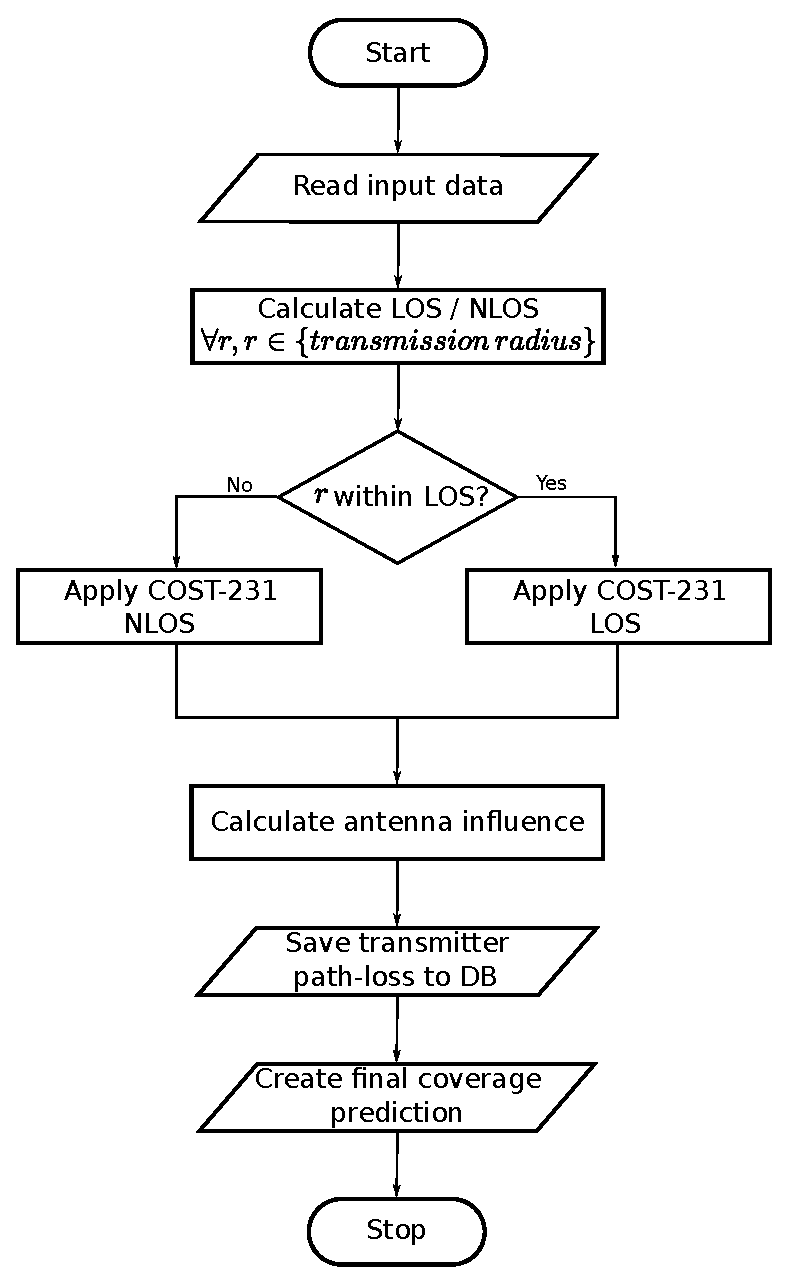
\includegraphics[width=1\columnwidth]{04-framework_design_and_implementation/img/serial_implementation_flow_diagram}

\caption{\textit{\emph{Flow diagram of the serial version.}}\textit{\label{fig:04-Flow_diagram_serial_version}}}
\end{figure}



\subsubsection{Isotropic path-loss calculation\label{sub:04-Isotrophic_pahloss_calculation}}

This step starts by calculating which receiver points, $r$, are within
the specified transmission radius (see ``\emph{transmission radius}''
in Figure~\ref{fig:04-Flow_diagram_serial_version}). The transmission
radius is defined around each transmitter in order to limit the radio-propagation
calculation to a reasonable distance. For these points, the path loss
for an isotropic source (or omni antenna) is estimated. This calculation
is performed by applying the radio-propagation model, which was previously
defined in Equation~(\ref{eq:04-Hata_pathloss}), to each of the
points within the transmission radius around the transmitter (see
``Calculate path loss'' in Figure~\ref{fig:04-Flow_diagram_serial_version}).

Figure~\ref{fig:04-Raster_path_loss_example} shows an example of
the isotropic path-loss calculation, only including the map area within
the transmission radius. The color scale is given in dB, indicating
the signal loss from the isotropic source of the transmitter, located
at the center. Notice the hilly terrain is clearly distinguished due
to LOS and NLOS conditions from the signal source.

\begin{figure}
\centering

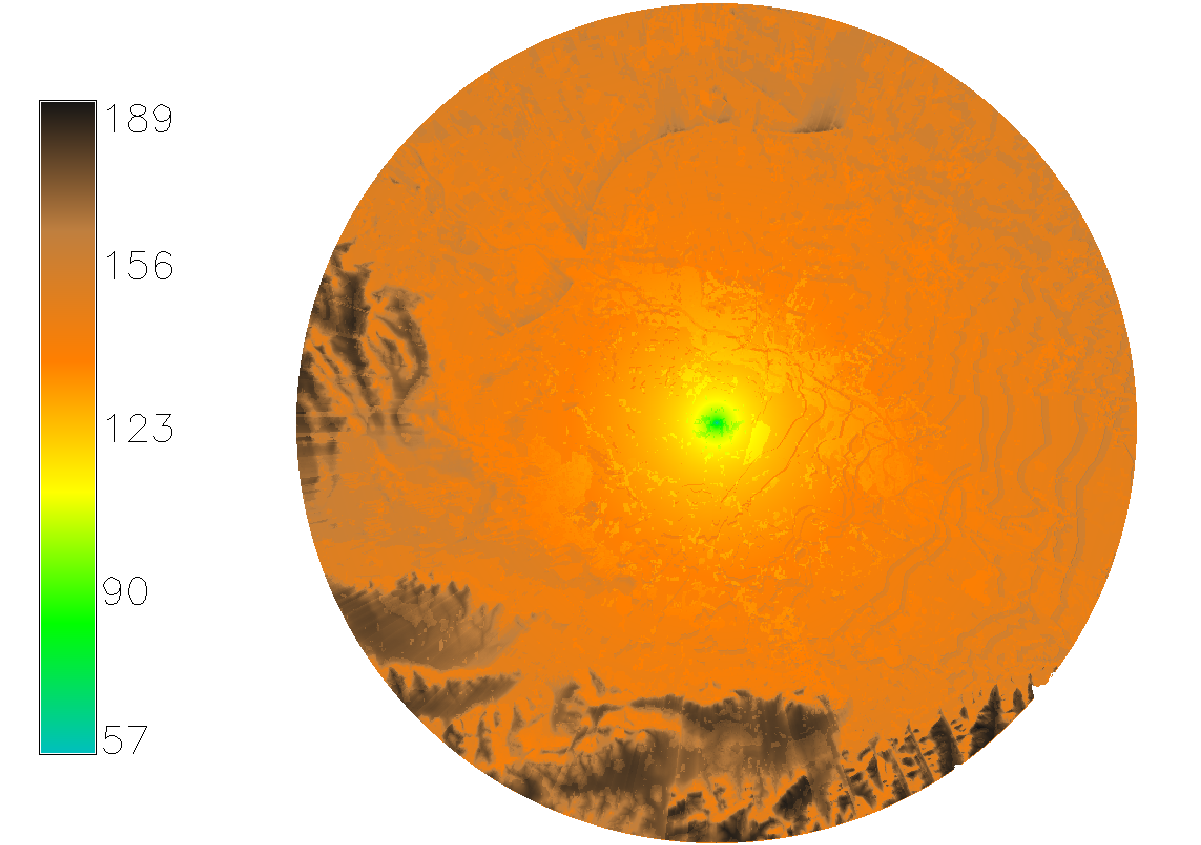
\includegraphics[width=0.6\textwidth]{04-framework_design_and_implementation/img/isotrophic_calculation}

\caption{\textit{\emph{Example of a raster map, showing the result of a path-loss
calculation from an isotropic antenna. The color scale is given in
dB, indicating the path loss at a given point. \label{fig:04-Raster_path_loss_example}}}}
\end{figure}



\subsubsection{Antenna diagram influence \label{sub:04-Antenna_diagram_influence}}

This step considers the antenna radiation diagram of the current transmitter
and its influence over the isotropic path-loss calculation (see ``Calculate
antenna influence'' in Figure~\ref{fig:04-Flow_diagram_serial_version}).
Working on the in-memory results generated by the previous step, the
radiation diagram of the antenna is taken into account, including
the beam direction, the electrical and the mechanical tilt. Figure~\ref{fig:04-Raster_antenna_example}
shows the map area within the transmission radius, where this calculation
step was applied to the results from Figure~\ref{fig:04-Raster_path_loss_example}.
Notice the distortion of the signal propagation that the antenna has
introduced.

\begin{figure}[h]
\centering

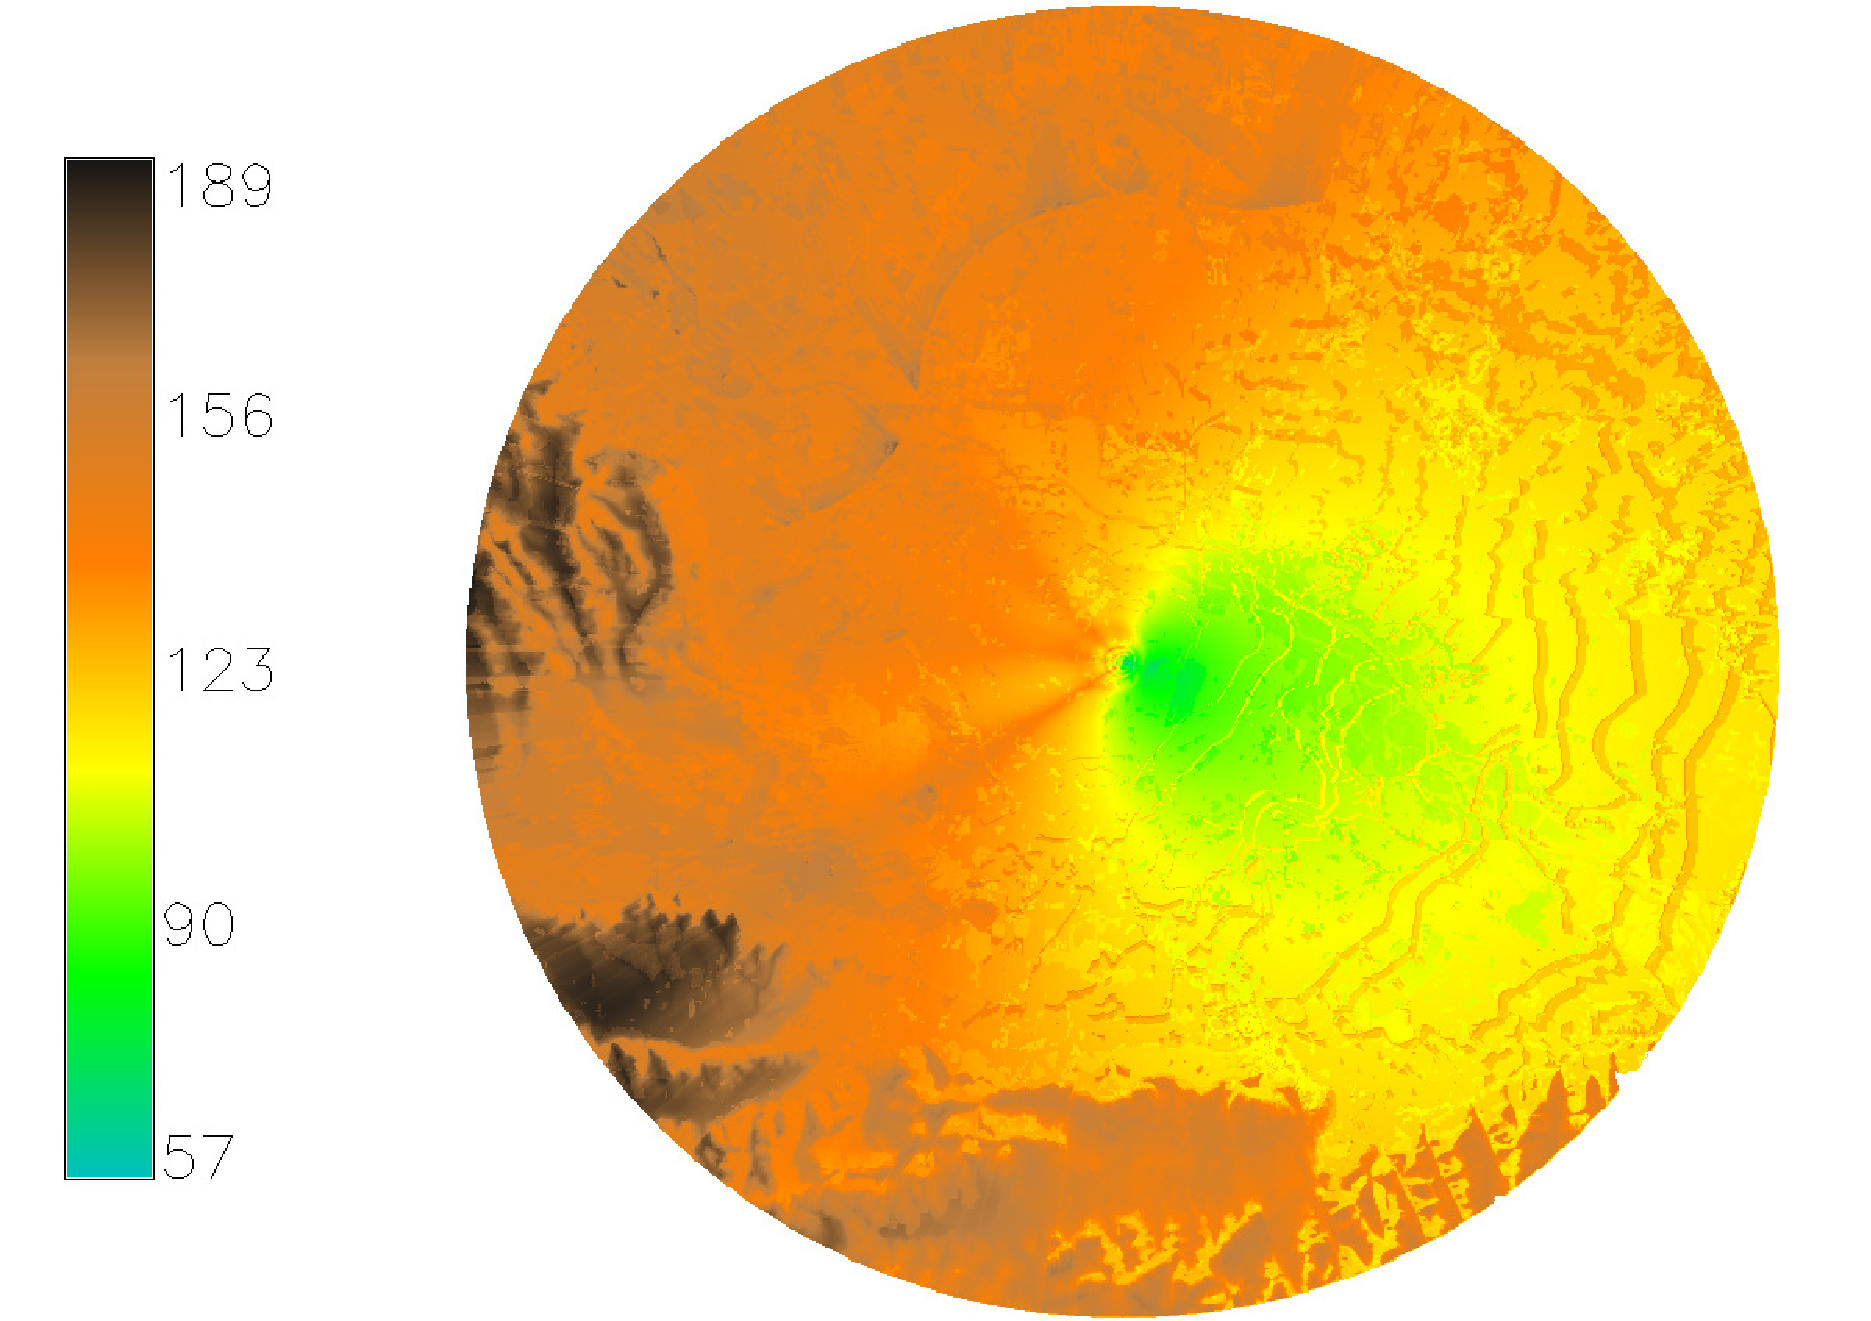
\includegraphics[width=0.6\textwidth]{04-framework_design_and_implementation/img/antenna_calculation}

\caption{\textit{\emph{Example of a raster map, showing the influence of a
directional antenna over the path-loss result depicted in Figure~\ref{fig:04-Raster_path_loss_example}.
The color scale is given in dB, indicating the path loss at a given
point. \label{fig:04-Raster_antenna_example}}}}
\end{figure}



\subsubsection{Transmitter path-loss prediction \label{sub:04-Transmitter_path_loss_prediction}}

In this step, the path-loss prediction of the transmitter is saved
in its own database table (see ``Save transmitter path-loss to DB''
in Figure~\ref{fig:04-Flow_diagram_serial_version}). This is accomplished
by connecting the standard output of the GRASS module with the standard
input of a database client. Naturally, the generated plain text should
be understood by the DB itself.


\subsubsection{Coverage prediction \label{sub:04-Coverage_prediction}}

\begin{figure}
\centering

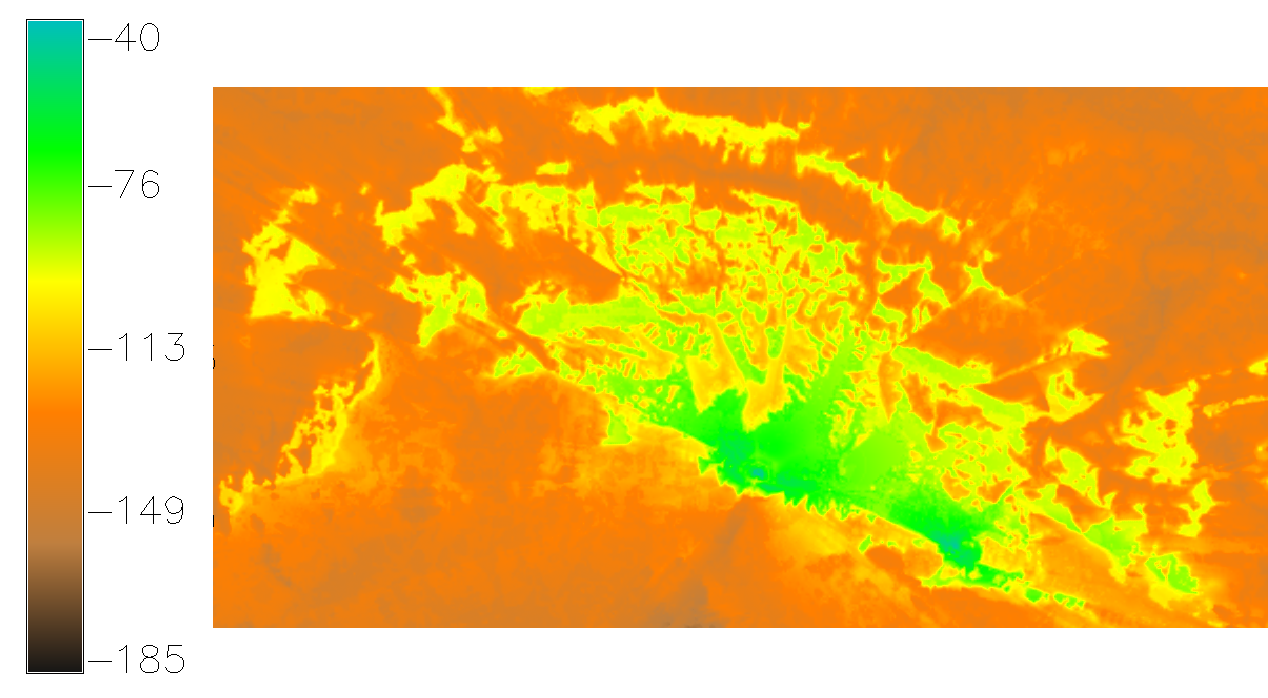
\includegraphics[width=0.65\textwidth]{04-framework_design_and_implementation/img/final_coverage}

\caption{\textit{\emph{Example of a raster map, displaying the final coverage
prediction of 136 transmitters over a geographical area. The color
scale is given in dBm, indicating the received-signal strength. Darker
colors denote areas with a reduced signal due to the fading effect
of the hilly terrain and clutter. \label{fig:04-Raster_prediction_example}}}}
\end{figure}


The final radio-coverage prediction, containing the aggregation of
the partial path-loss results of the involved transmitters, is created
in this step (see ``Create final coverage prediction'' in Figure~\ref{fig:04-Flow_diagram_serial_version}).
The received signal strength from each of the transmitters is calculated
as the difference between its transmit power and the path loss for
the receiver's corresponding position. This is done by executing an
SQL query over the tables containing the path-loss predictions of
each of the processed transmitters. Finally, the output is generated
using the GRASS built-in modules $v.in.ascii$ and $v.to.rast$, which
create a raster map using the query results as the input. The resulting
raster map contains the maximum received signal strength for each
individual point, as shown in Figure~\ref{fig:04-Raster_prediction_example}.
In this case, the color scale is given in dBm, indicating the strongest
received signal strength from the transmitters.


\subsection{Computational complexity \label{sub:04-Computational_complexity}}

\begin{algorithm}
\centering

\caption{Pseudo-code of the radio-coverage prediction algorithm. The time complexity
is given per line.\label{alg:04-Pseudocode_radio_coverage_algorithm}}


\begin{algorithmic}
\State $DEM \gets$ DEM of the whole area.
\Comment $O(M)$
\State $Clutter \gets$ signal losses due to clutter of the whole area.
\Comment $O(M)$
\State $T \gets$ transmitter configuration data.
\Comment $O(n)$
\ForAll{$t \in T$}
	\Comment $O(n \cdot m^2)$
	\State $DEM_{t} \gets $ DEM area within transmission radius of ${t}$
	\Comment $O(m)$
	\State $Clut_{t} \gets $ Clutter area within transmission radius ${t}$
	\Comment $O(m)$
	\State $LoS_{t} \gets$ LineOfSight ($DEM_{t}$)
	\Comment $O(m^2)$
	\State $PL_{t} \gets$ PathLoss ($DEM_{t}, Clut_{t}, LoS_{t}$)
	\Comment $O(m^2)$
	\State $Diag_{t} \gets $ Antenna diagram of ${t}$ 
	\Comment $O(1)$
	\State $PL_{t} \gets$ AntennaInfluence ($Diag_{t}, PL_{t}$)
	\Comment $O(m)$
\EndFor
\ForAll{$t \in T$}
	\Comment $O(n \cdot m)$
	\State $CoveragePrediction \gets$ PathLossAggregation ($t, PL_{t}$)
	\Comment $O(m)$
\EndFor
\State \Return $CoveragePrediction$
\end{algorithmic}
\end{algorithm}


In this section, the time complexity of the radio-coverage prediction
algorithm is presented, the pseudo-code of which is \textit{\emph{listed}}
in Algorithm~\ref{alg:04-Pseudocode_radio_coverage_algorithm}.

The algorithm starts by loading the input DEM and clutter data. Both
RSGs should account for the same area and resolution, consequently
containing the same number of pixels, $M$. The transmitter data is
then loaded into set $T$, the cardinality of which is denoted as
$n=|T|$. For each transmitter $t\in T$, a smaller subarea of the
DEM and clutter data, denoted as $DEM_{t}$ and $Clut_{t}$, respectively,
is delimited around $t$, based on a given transmission radius. The
number of pixels within this sub-area is denoted as $m$, and its
value is the same for all $t\in T$. The visibility for an RSG pixel
is computed using the \emph{LineOfSight} function, by walking from
the antenna of the transmitter to the given pixel element, along the
elements intersected by a LOS, until either the visibility is blocked,
or the target is reached~\cite{DeFloriani-Applications_of_computational_geometry_to_geographic_information_systems:1999}.
Regarding the \emph{PathLoss }function, whenever a receiver point
is in NLOS, the walking path from the transmitter has to be inspected
for obstacles, calculating the diffraction losses for each of them,
i.e., $\alpha$ and $K(d_{(x,y)})$ from Equation~(\ref{eq:04-Hata_NLOS}).
Hence, its quadratic complexity, which dominates the complexity of
the algorithm, together with \emph{LineOfSight}, resulting in an algorithmic
complexity denoted by:

\begin{equation}
O(M+n\cdot m^{2}).
\end{equation}


\noindent On the one hand, $n$ will generally be many orders of magnitude
smaller than $m^{2}$, although its computational-time complexity
is relevant for practical use. For example, assuming the radio-coverage
prediction for one transmitter completes in around 15~seconds using
a serial implementation, the prediction for a mobile network comprising
10,240 transmitters would have an execution time of almost two days.
On the other hand, when the input data correspond to a large geographical
area, and only one transmitter is selected with a narrow calculation
radius, i.e., $M$ is large, $n=1$ and $m$ is small, then $O(M)$
will donimate the time complexity of the algorithm.


\subsection{Design of the parallel version \label{sub:04-Design_of_the_parallel_version}}

The focus here is on the practical usability and performance of PRATO.
The parallel implementation aims at overcoming the computational-time
constraints that prevent a serial implementation from tackling bigger
problem instances in a feasible amount of time.

A major drawback of the GRASS as a parallelization environment is
that it is not thread-safe, meaning that concurrent changes to the
same data set have an undefined behavior~\cite{Blazek_GRASS_server:2004}.
One technique to overcome this problem is to abstract the spatial
data from the GRASS. For example, in~\cite{Huang-Explorations_of_the_implementation_of_a_parallel_IDW_algorithm_in_a_Linux_cluster:2011},
the authors achieved the GRASS abstraction by introducing a \emph{Point
}structure with four \emph{double} attributes, where each pixel of
the RSG is mapped to an instance of this structure. Another possibility
is for one of the processes, e.g., the master, to read entire rows
or columns of data before dispatching them for processing to the workers
\cite{Akhter_Porting_GRASS_raster_module_to_distributed_computing:2007,Huang-Explorations_of_the_implementation_of_a_parallel_IDW_algorithm_in_a_Linux_cluster:2011}.
In this case, an independence between row/column calculations is required,
which is a problem-specific property. Here, abstraction from the GRASS
is achieved by loading each spatial-data set into a separate 2D matrix
of basic data-type elements, e.g., \emph{float} or \emph{double} depending
on the desired accuracy. Each matrix is then assigned the geographical
location of the closest corner to the origin of the map-projection
system used, e.g., the lower-left corner for the transverse Mercator
map projection over central Europe. It follows that the geographical
location of any element within the matrix is calculated as the combination
of the geographical location of the matrix and the offset of the target
element (see Figure~\ref{fig:04-Spatial_data_location_mapping}).
The advantage of this technique is having the geographical location
of a pixel readily available with a minimum memory footprint. Moreover,
a convenient consequence of this abstraction schema is that worker
processes are completely independent of the GRASS, thus significantly
simplifying the deployment of the parallel implementation over multiple
computing hosts.

\begin{figure}
\centering

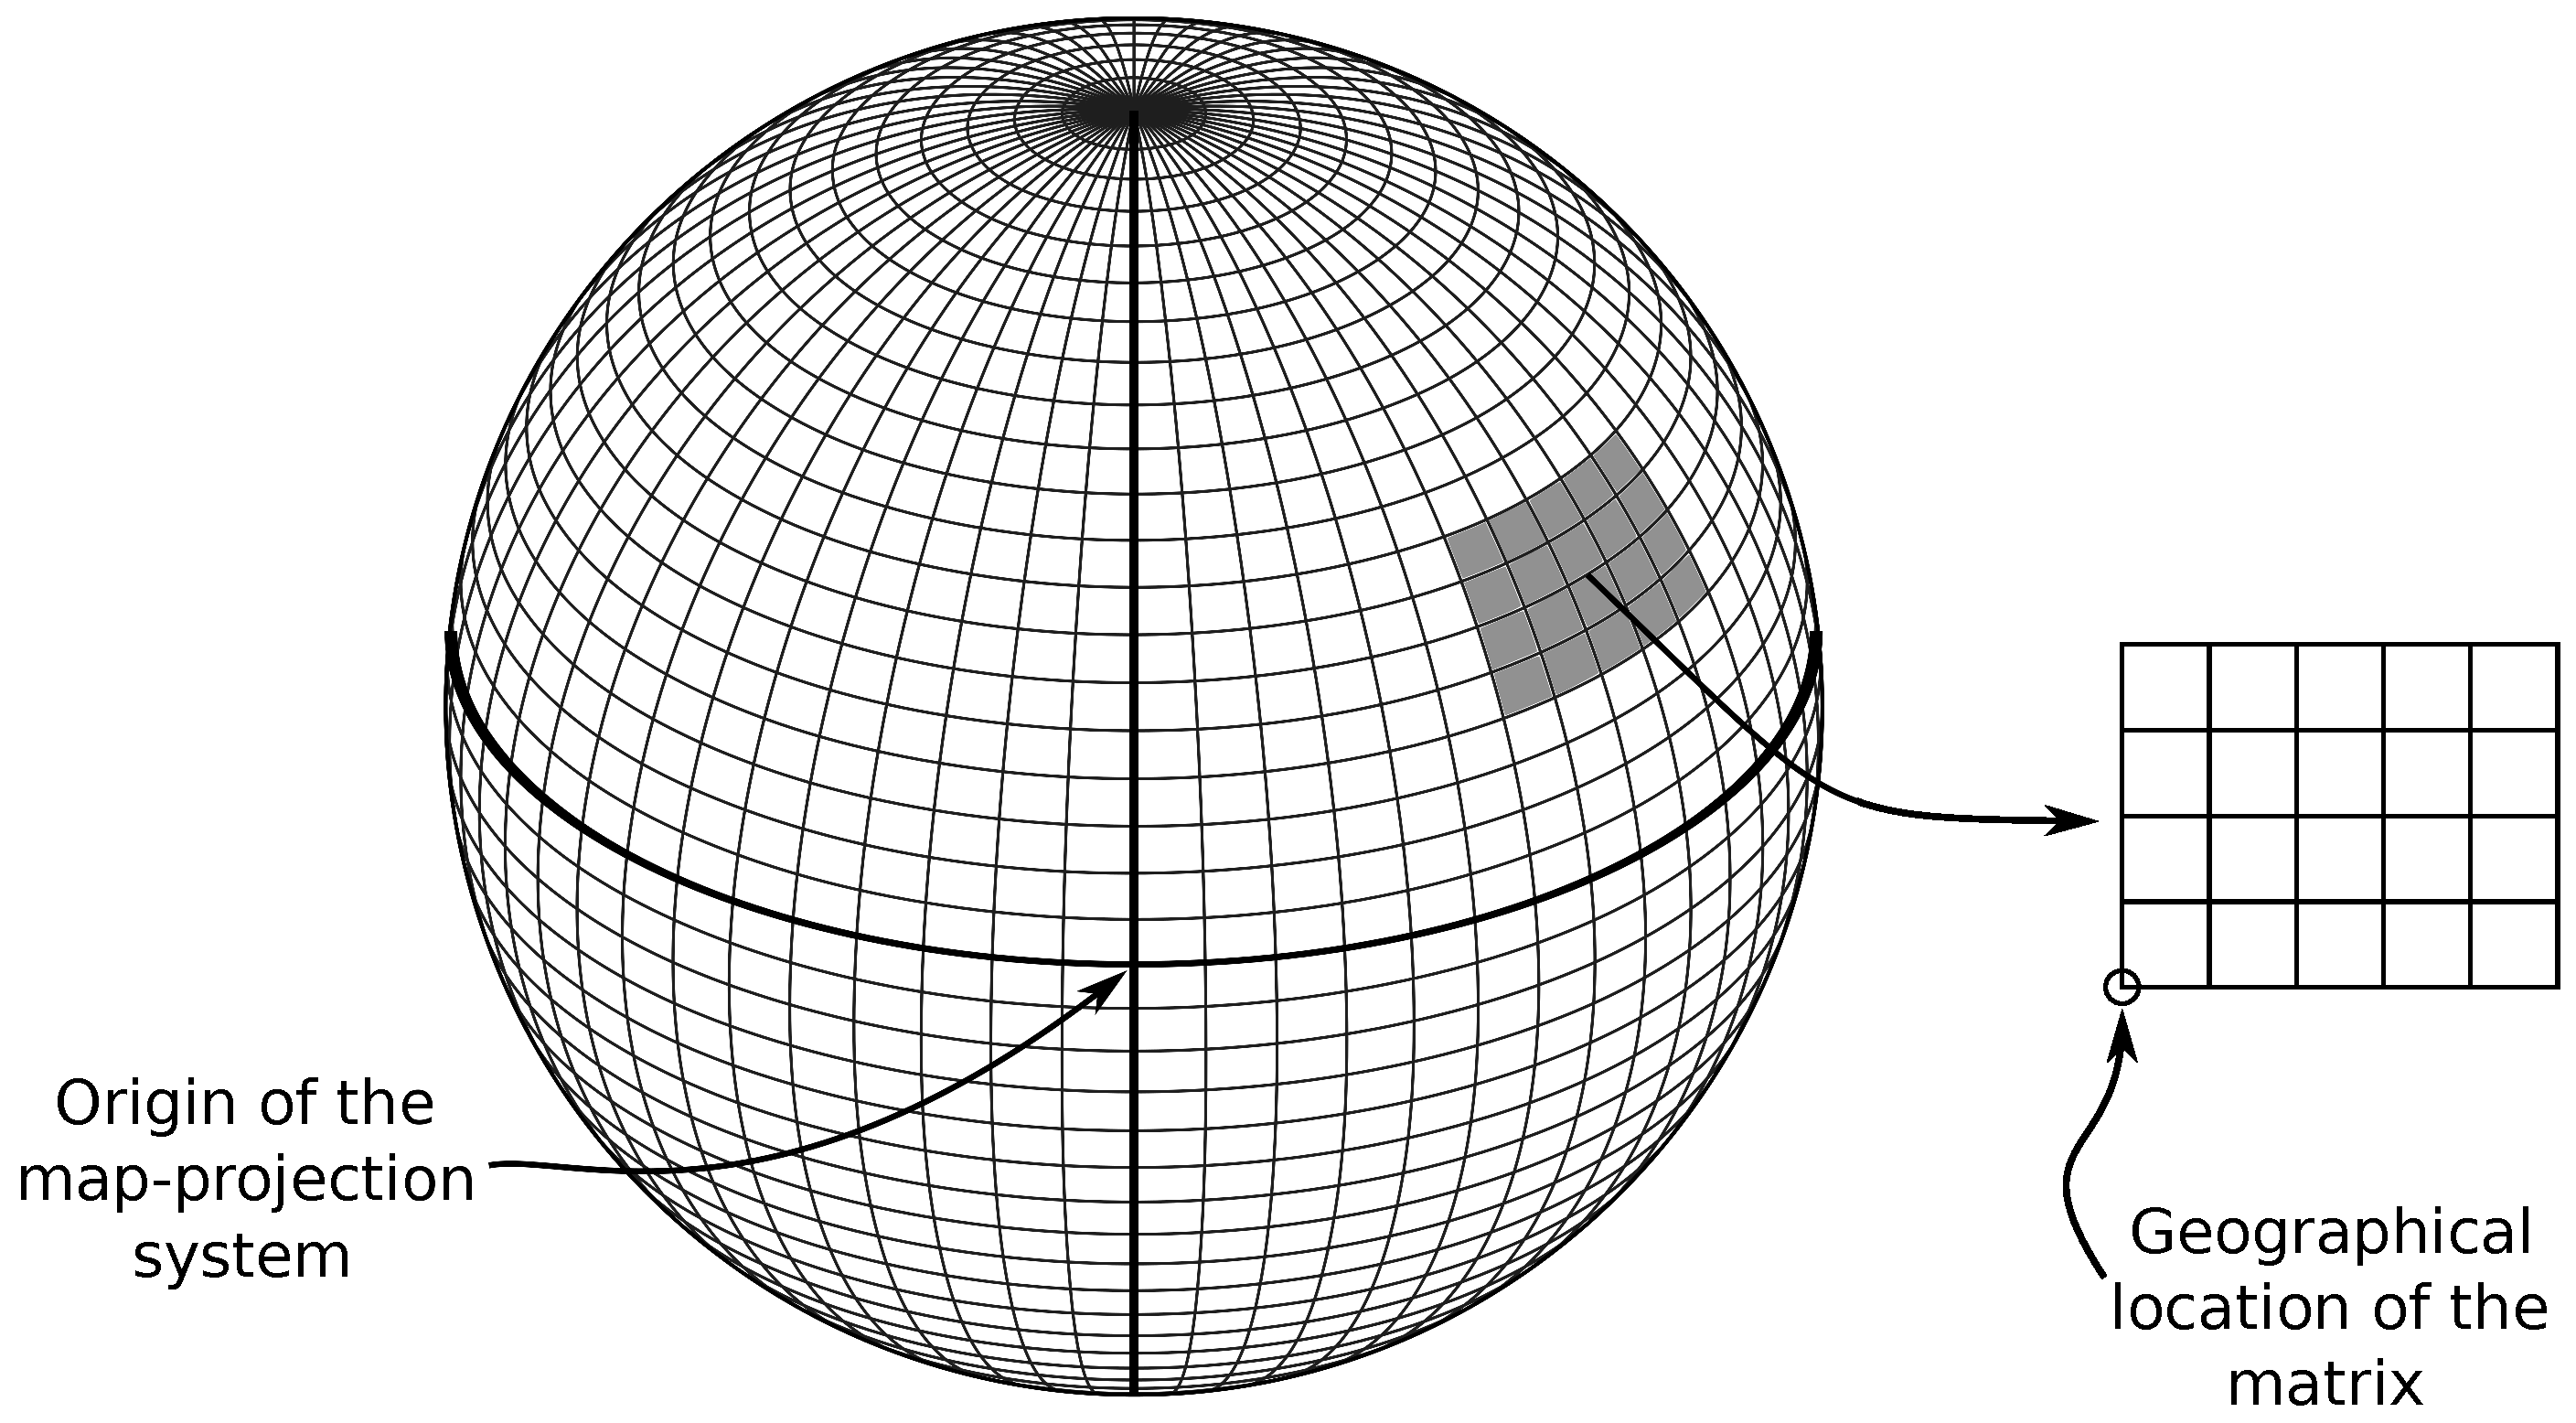
\includegraphics[width=1\textwidth]{04-framework_design_and_implementation/img/spatial_data_projection}

\caption{Example of a geographical-location mapping of the input-spatial data
into a 2D matrix, the lower-left corner of which indicates the nearest
point to the origin of the map-projection system.\label{fig:04-Spatial_data_location_mapping}}
\end{figure}


In the area of geographical-information science, the master-worker
paradigm has been successfully applied by several authors~\cite{Akhter-GRASS_GIS_on_high_performance_computing_with_MPI_OpenMP_and_Ninf-G:2010,Akhter_Porting_GRASS_raster_module_to_distributed_computing:2007,Campos_Parallel_modelling_in_GIS:2012,Guan_A_parallel_computing_approach_to_fast_geostatistical_areal_interpolation:2011,Huang-Explorations_of_the_implementation_of_a_parallel_IDW_algorithm_in_a_Linux_cluster:2011,Tabik-High_performance_three_horizon_composition_algorithm_for_large_scale_terrains:2011,Tabik-Optimal_tilt_and_orientation_maps_a_multi_algorithm_approach_for_heterogeneous_multicore_GPU_systems:2013}.
However, this technique presents certain issues that prevent the full
exploitation of the available computing resources when deployed over
several networked computers. Specifically, the problem refers to network
saturation and idle processes within the master-worker model. Generally
speaking, a single communicating process, e.g., the master, is usually
not able to saturate the network connection of a node. Using more
than one MPI process per node might solve this problem, but possible
rank-ordering problems may appear, thus restricting the full utilization
of the network~\cite{Rabenseifner-Hybrid_MPI_OpenMP_parallel_programming_on_clusters_of_multicore_nodes:2009}.
Additionally, the hardware-exploitation level is difficult to measure
when the parallelization involves only one computing node~\cite{Tabik-High_performance_three_horizon_composition_algorithm_for_large_scale_terrains:2011,Tabik-Optimal_tilt_and_orientation_maps_a_multi_algorithm_approach_for_heterogeneous_multicore_GPU_systems:2013}
(because no network communication is required), or only a few processes
deployed over a handful of nodes~\cite{Huang-Explorations_of_the_implementation_of_a_parallel_IDW_algorithm_in_a_Linux_cluster:2011}. 

Another issue appears when the master process executes the MPI code,
in which case other processes sleep, making a serial use of the communication
component of the system. Consequently, the master process becomes
the bottleneck of the parallel implementation as the number of worker
processes grows. This situation is also common when dealing with the
metadata of a spatial region, which may relate to several elements
of a RSG, making it a frequent cause of load imbalance~\cite{Gong_Parallel_agent_based_simulation_of_individual_level_spatial_interactions_within_a_multicore_computing_environment:2012,Hawick_Distributed_frameworks_and_parallel_algorithms_for_processing_large_scala_geographic_data:2003,Widener_Developing_a_parallel_computational_implementation_of_AMOEBA:2012}.
In PRATO, the transmitter configuration and its antenna diagram represent
metadata that are complementary to the sub-region that a transmitter
covers.

Hybrid MPI-OpenMP implementations~\cite{Tabik-High_performance_three_horizon_composition_algorithm_for_large_scale_terrains:2011,Tabik-Optimal_tilt_and_orientation_maps_a_multi_algorithm_approach_for_heterogeneous_multicore_GPU_systems:2013},
in which no MPI calls are issued inside the OpenMP-parallel regions,
also fail to saturate the network~\cite{Rabenseifner-Hybrid_MPI_OpenMP_parallel_programming_on_clusters_of_multicore_nodes:2009}.
A possible solution to this problem is to improve the communication
overlap among the processes. To this end, PRATO features non-blocking
point-to-point MPI operations, and an independent thread in the worker
process that saves the intermediate results into a DB. One such database
system per computer cluster is used, which also serves the input data
to the GRASS, in order to aggregate the partial results of the path-loss
predictions or to visualize them. It is important to note that any
kind of DB may be used, e.g., relational, distributed~\cite{Ozsu_Principles_of_distributed_database_systems:2011}
or even those of the NoSQL type~\cite{Stonebraker_SQL_databases_vs_NoSQL_databases:2010}.
Nevertheless, a central, relational-database system is used here,
since they are the most popular and widely available ones. Additionally,
the non-blocking message-passing technique used to distribute the
work-load among the nodes provides support for heterogeneous environments.
As a result, computing nodes featuring more capable hardware receive
more work than those with weaker configurations, thus ensuring a better
utilization of the available computing resources despite hardware
diversity, and improved load balancing.


\subsubsection{Master process \label{sub:04-Master-process}}

\begin{figure}
\begin{minipage}[t]{0.49\textwidth}%
\centering

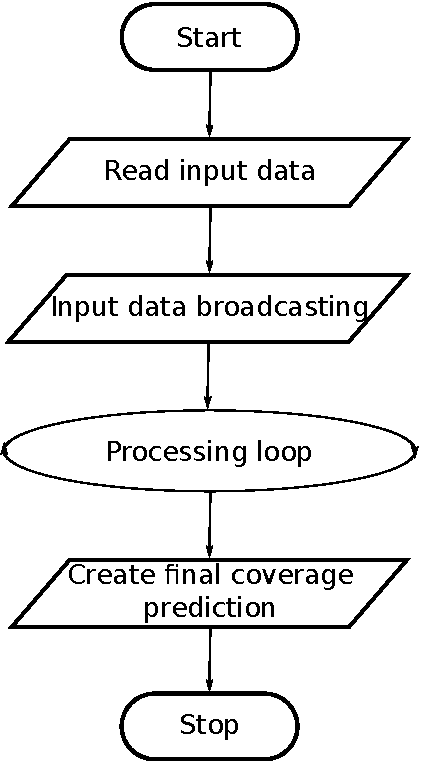
\includegraphics[width=0.55\columnwidth]{04-framework_design_and_implementation/img/master_process_flow_diagram}

\caption{\textit{\emph{Flow diagram of the master process.\label{fig:04-Master_process_flow_diagram}}}}
%
\end{minipage}\hfill{}%
\begin{minipage}[t]{0.49\textwidth}%
\centering

\includegraphics[width=1\columnwidth]{04-framework_design_and_implementation/img/master_processing_loop_flow_diagram}

\caption{\textit{\emph{Flow diagram of the ``Processing loop'' step of the
master process.\label{fig:04-Processing_loop_in_master_process}}}}
%
\end{minipage}
\end{figure}


The master process, the flow diagram of which is given in Figure~\ref{fig:04-Master_process_flow_diagram},
is the only component that runs within the GRASS environment. As soon
as the master process starts, the input parameters are read. This
step corresponds to ``Read input data'' in Figure~\ref{fig:04-Master_process_flow_diagram},
and it is carried out in a similar way as in the serial version. The
next step delivers the metadata that is common to all the transmitters
to all the processes (see ``Metadata broadcasting'' in Figure~\ref{fig:04-Master_process_flow_diagram}).
Before distributing the work among the worker processes, the master
process proceeds to decompose the loaded raster data into 2D matrices
of basic-data-type elements, e.g., \emph{float} or \emph{double},
before dispatching them to the multiple worker processes. In this
case, the decomposition applies to the DEM and the clutter data only,
but it could be applied to any point-based data set. In the next step,
the master process starts an asynchronous message-driven processing
loop (see ``Processing loop'' in Figure~\ref{fig:04-Master_process_flow_diagram}),
the main task of which is to assign and distribute the sub-region
and configuration data of different transmitters among the idle worker
processes.

The flow diagram shown in Figure~\ref{fig:04-Processing_loop_in_master_process}
illustrates the ``Processing loop'' step of the master process.
In the processing loop, the master process starts by checking the
available worker processes, that might calculate the radio-coverage
prediction for the next transmitter. It is worth pointing out that
this step also serves as a stopping condition for the processing loop
itself (see ``Any worker still on?'' in Figure~\ref{fig:04-Processing_loop_in_master_process}).
The active worker processes inform the master process that they are
ready to compute by sending an idle message (see ``Wait for idle
worker'' in Figure~\ref{fig:04-Processing_loop_in_master_process}).
The master process then announces to the idle worker process that
it is about to receive new data for the next calculation, and it dispatches
the complete configuration of the transmitter to be processed (see
``Send keep-alive message'' and ``Send transmitter data'' steps,
respectively, in Figure~\ref{fig:04-Processing_loop_in_master_process}).
This is only done in the case that there are transmitters for which
the coverage prediction has yet to be calculated (see ``Any transmitters
left?'' in Figure~\ref{fig:04-Processing_loop_in_master_process}).
The processing loop of the master process continues distributing the
transmitter data among the worker processes, which asynchronously
become idle as they finish the radio-prediction calculations they
have been assigned by the master process. When there are no more transmitters
left, all the worker processes announcing they are idle will receive
a shutdown message from the master process, indicating to them that
they should stop running (see ``Send stop message'' in Figure~\ref{fig:04-Processing_loop_in_master_process}).
The master process will keep doing this until all the worker processes
have finished (see ``Any worker still on?'' in Figure~\ref{fig:04-Processing_loop_in_master_process}),
thus fulfilling the stopping condition of the processing loop.

Finally, the last step of the master process is devoted to creating
the final output of the calculation, e.g., a raster map (see ``Create
final coverage prediction'' in Figure~\ref{fig:04-Master_process_flow_diagram}).
The final coverage prediction of all the transmitters is an aggregation
from the individual path-loss results created by each of the worker
processes during the ``Processing loop'' phase in Figure~\ref{fig:04-Master_process_flow_diagram},
which provides the source data for the final raster map. The aggregation
of the individual path-loss results is accomplished by issuing an
SQL query over the database tables containing them, in a similar way
as in the serial version.


\subsubsection{Worker processes on CPU}

An essential characteristic of the worker processes is that they are
completely independent of the GRASS, i.e., they do not have to run
within the GRASS environment nor use any of the GRASS libraries to
work. This aspect significantly simplifies the deployment phase to
run PRATO on a computer cluster, since no GRASS installation is needed
on the computing nodes hosting the worker processes.

One possibility to overcome the thread-safety limitation of the GRASS
is to save the transmitter path-loss predictions through the master
process, thus avoiding concurrent access. However, for the workers
to send intermediate results back to the master process, e.g., as
in~\cite{Akhter-GRASS_GIS_on_high_performance_computing_with_MPI_OpenMP_and_Ninf-G:2010,Huang-Explorations_of_the_implementation_of_a_parallel_IDW_algorithm_in_a_Linux_cluster:2011},
is a major bottleneck for the scalability of a parallel implementation.
In such case, the scalability is limited by the master process, because
it must serially process the received results in order to avoid inconsistencies
due to concurrent access. Instead, PRATO allows each of the worker
processes to output its intermediate results into a DB, i.e., each
path-loss prediction in its own table. Additionally, worker processes
do this from an independent thread, which runs concurrently with the
calculation of the next transmitter received from the master process.
In this way, the overlap between the calculation and communication
significantly hides the latency created by the result-dumping task,
thus making better use of the available system resources.

The computations of the worker processes, the flow diagram of which
is given in Figure~\ref{fig:04-Worker_process_flow_diagram}, begin
by receiving metadata about the transmitters and the geographical
area from the master process during the initialization time (see ``Receive
broadcasted metadata'' in Figure~\ref{fig:04-Worker_process_flow_diagram}).

After the broadcasted metadata are received by all the worker processes,
each one proceeds to inform the master process that it is ready (i.e.,
in an idle state) to receive the transmitter-configuration data that
define which transmitter path-loss prediction to perform (see ``Send
idle message'' in Figure~\ref{fig:04-Worker_process_flow_diagram}).
If the master process does not give the instruction to stop processing
(see ``Has stop message arrived?'' in Figure~\ref{fig:04-Worker_process_flow_diagram}),
the worker process collects the sub-region spatial data and the transmitter
configuration (see ``Receive transmitter data'' in Figure~\ref{fig:04-Worker_process_flow_diagram}).
In the event that a stop message is received, the worker process will
wait for any result-dumping thread to finish (see ``Wait for result-dump
thread'' in Figure~\ref{fig:04-Worker_process_flow_diagram}) before
shutting down. The coverage calculation itself follows a similar design
as the serial version (see ``Coverage calculation'' in Figure~\ref{fig:04-Worker_process_flow_diagram}).

As mentioned before, the worker process launches an independent thread
to save the path-loss prediction of the target transmitter into a
DB table (see ``Threaded save path-loss to DB'' in Figure~\ref{fig:04-Worker_process_flow_diagram}).
It is important to note that there is no possibility of data inconsistency
due to the saving task being executed inside a thread, since path-loss
data from different workers belong to different transmitters and are,
at this point of the process, mutually exclusive.

\begin{figure}
\begin{minipage}[t]{0.49\textwidth}%
\centering

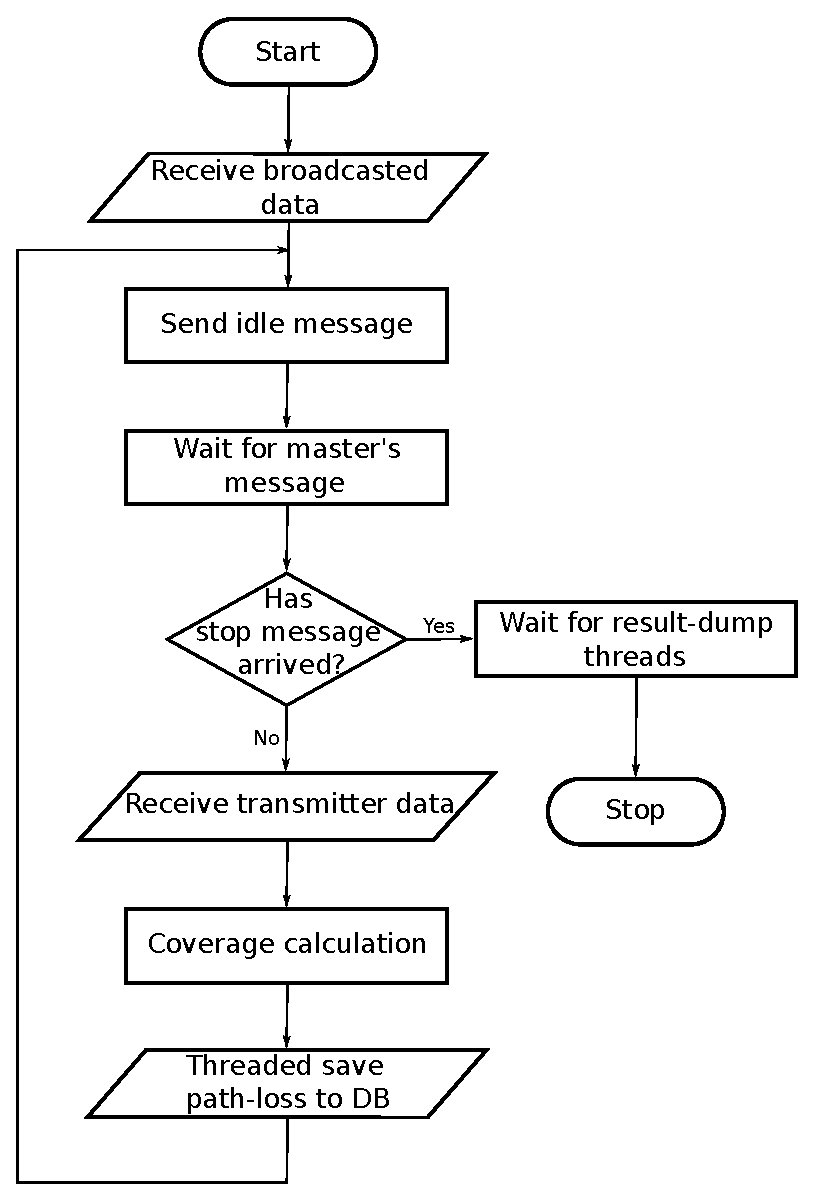
\includegraphics[width=0.9\columnwidth]{04-framework_design_and_implementation/img/worker_process_flow_diagram}

\caption{\textit{\emph{Flow diagram of a worker process.\label{fig:04-Worker_process_flow_diagram}}}}
%
\end{minipage}\hfill{}%
\begin{minipage}[t]{0.49\textwidth}%
\centering

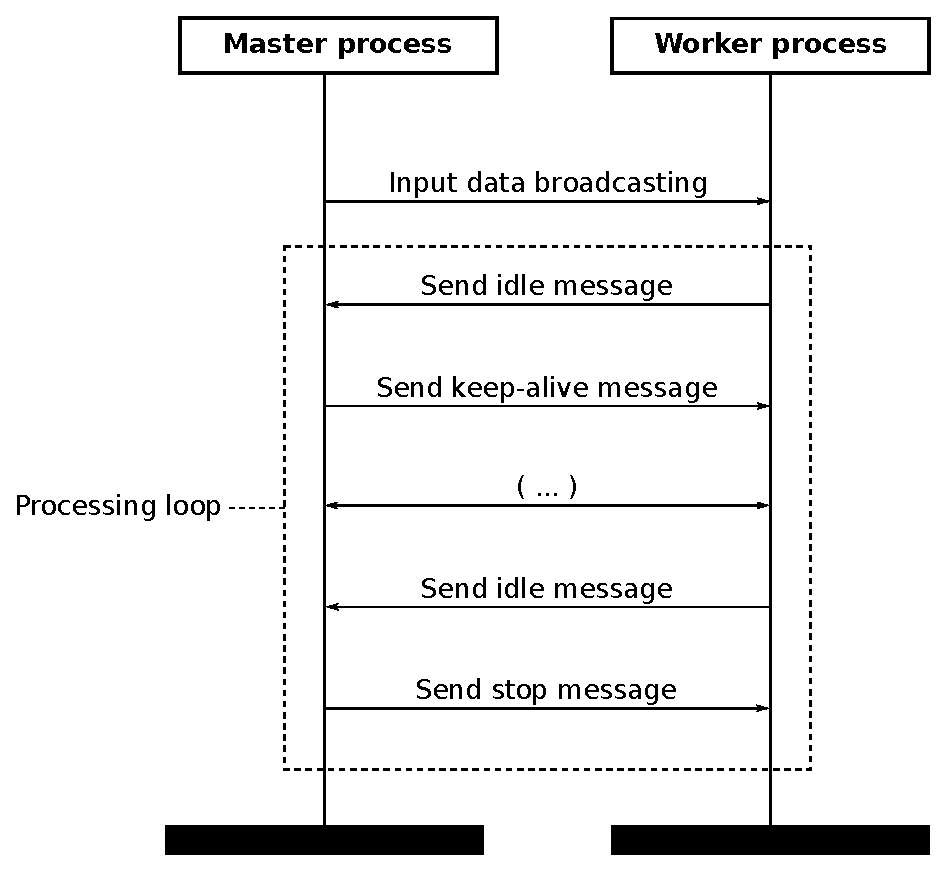
\includegraphics[width=1\columnwidth]{04-framework_design_and_implementation/img/master_worker_communication_diagram}

\caption{\textit{\emph{Communication diagram, showing the message passing between
the master and a worker process.\label{fig:04-Master_worker_communication}}}}
%
\end{minipage}
\end{figure}



\subsubsection{Worker processes on GPU \label{sub:04-GPU_worker_implementation}}

PRATO provides multi-GPU support for improving the execution performance
on the computing nodes hosting the worker processes. The algorithmic
adaptation from a CPU to a GPU is not a trivial task. This section
focuses on the main modifications made to the radio-propagation algorithm
in order for it to work on GPU hardware.

It is well known that the bandwidth of the PCI Express bus can cause
a throughput bottleneck when a significant amount of data is transferred
between a CPU and a GPU in a heterogeneous system~\cite{Gregg-Where_is_the_data:2011}.
Some researchers acknowledged that unless a full working set of data
can fit into the memory on a GPU, the PCI Express will become the
bottleneck of the system~\cite{Owens-GPU_computing:2008,Schaa-Exploring_the_multiple_GPU_design_space:2009}.
For this reason, it is imperative to have as much data as possible
allocated on the GPU itself.

In order to minimize the CPU-to-GPU memory transfers, the spatial
data used by the radio-propagation algorithm was organized as explained
in Section~\ref{sub:04-Design_of_the_parallel_version}, i.e., using
geographically-located, offset-based 2D matrices. However, the internal
representation of the matrix elements was changed to use less memory.
To this end, the clutter-matrix elements were represented as \emph{unsigned
char}, since they express signal loss in dB. It follows that for the
radio-propagation prediction of one transmitter, the following matrices
should be allocated on the GPU:
\begin{itemize}
\item one 2D matrix containing DEM data for the target subregion, the elements
of which are \emph{float} or \emph{double}; 
\item one 2D matrix containing clutter data for the target subregion, the
elements of which are \emph{unsigned char}; and
\item one 2D matrix containing the resulting path-loss prediction.
\end{itemize}
The dimension of all matrices is based on the transmission radius,
within which the radio-propagation prediction should be calculated.
The contents of the DEM and clutter matrices is constant throughout
the calculation process. For this reason they were kept in texture
memory to take advantage of the faster access time (see Section~\ref{sec:02-CUDA}).
Regarding the resulting path-loss matrix, each step of the radio-prediction
algorithm is applied over the results of the previous step (see Figure~\ref{fig:04-Flow_diagram_serial_version}
for a flow diagram of the steps involved), thus avoiding extra allocation
on global memory or a data-transfer from/to the CPU.


\subsubsection{Master-worker communication}

Similar to~\cite{Tabik-High_performance_three_horizon_composition_algorithm_for_large_scale_terrains:2011,Tabik-Optimal_tilt_and_orientation_maps_a_multi_algorithm_approach_for_heterogeneous_multicore_GPU_systems:2013},
the message-passing technique used in this work enables a better use
of the available computing resources, both in terms of scalability
and load balancing, while introducing a negligible overhead. This
last point is supported by the experimental results, introduced in
Section~\ref{sub:04-Strong_scalability}.

The first reason to implement the message-passing technique is to
support heterogeneous computing environments. In particular, our approach
focuses on taking full advantage of the hardware of each computing
node, thus explicitly avoiding the bottlenecks introduced by the slowest
computing node in the cluster. This problem appears when evenly distributing
the data among the worker processes on disparate hardware, e.g., as
in~\cite{Akhter_Porting_GRASS_raster_module_to_distributed_computing:2007,Huang-Explorations_of_the_implementation_of_a_parallel_IDW_algorithm_in_a_Linux_cluster:2011},
being more noticeable with a larger number of computing nodes and
processes. In other words, computing nodes that deliver better performance
have more calculations assigned to them. Moreover, in real-world scenarios,
it is often the case that a large number of dedicated computing nodes
featuring exactly the same configuration is difficult to find, i.e.,
not every organization owns a computer cluster.

A second reason for selecting a message-passing technique is related
to the flexibility it provides for load balancing, which is of greater
importance when dealing with extra data or information besides spatial
data~\cite{Hawick_Distributed_frameworks_and_parallel_algorithms_for_processing_large_scala_geographic_data:2003}.
This can be seen in Figure~\ref{fig:04-Processing_loop_in_master_process},
where the master process, before delivering the spatial subset and
transmitter-configuration data, sends a message to the worker process,
indicating that it is about to receive more work. This a priori meaningless
message plays a key role in correctly supporting the asynchronous
process communication. Notice that the subset of spatial data that
a worker process receives is directly related to the transmitter for
which the prediction will be calculated. Similar to~\cite{Tabik-High_performance_three_horizon_composition_algorithm_for_large_scale_terrains:2011,Tabik-Optimal_tilt_and_orientation_maps_a_multi_algorithm_approach_for_heterogeneous_multicore_GPU_systems:2013},
this problem-specific property enables the use of a data-decomposition
technique based on a block partition of spatial data, e.g., the DEM
and clutter data.

In general, there are many different ways a parallel program can be
executed, because the steps from the different processes can be interleaved
in various ways and a process can make non-deterministic choices~\cite{Siegel_Verification_of_halting_properties_for_MPI_programs:2007},
which may lead to situations such as race conditions~\cite{Clemencon_MPI_Race_detection:1995}
and deadlocks. A deadlock occurs whenever two or more running processes
are waiting for each other to finish, and thus neither ever does.
To prevent PRATO from deadlocking, message sending and receiving should
be paired, i.e., an equal number of send and receive messages on the
master and worker sides~\cite{Siegel_Verification_of_halting_properties_for_MPI_programs:2007}.
Figure~\ref{fig:04-Master_worker_communication} depicts the master-worker
message passing, from which the transmitter-data transmission has
been excluded for clarity. Notice how each idle message sent from
the worker process is paired with an answer from the master process,
whether it is a keep-alive or a stop message.


\section{Simulations \label{sec:04-Simulations}}

Considering the large computational power needed for predicting the
radio-coverage of a real radio network, the use of a computer cluster
is recommended. A computer cluster is a group of interconnected computers
that work together as a single system. Computer clusters typically
consist of several commodity PCs connected through a high-speed local-area
network (LAN\nomenclature[A]{LAN}{Local area network.}) with a distributed
file system, like the network file system (NFS\nomenclature[A]{NFS}{Network file system.})~\cite{Shepler_Network_file_system:2003}.
One such system is the DEGIMA cluster \cite{Hamada_Cluster_of_GPUs:2010}
at the Nagasaki Advanced Computing Center (NACC\nomenclature[A]{NACC}{Nagasaki advanced computing center.})
of the Nagasaki University in Japan. This system ranked in the TOP
500 list of supercomputers until June 2012%
\footnote{http://www.top500.org%
}, and in June 2011 it held the third place in the Green 500 list%
\footnote{http://www.green500.org%
} as one of the most energy-efficient supercomputers in the world.

This section presents the simulations, and an exhaustive analysis
of the performance and scalability of the parallel implementation
of PRATO. The most common usage case for PRATO is to perform a radio-coverage
prediction for multiple transmitters. Therefore, a straight-forward
parallel decomposition is to divide a given problem instance by transmitter,
for which each coverage prediction is calculated by a separate worker
process.

The following simulations were carried out on 34 computing nodes of
the DEGIMA cluster. The computing nodes are connected by a LAN, over
a Gigabit Ethernet interconnect. As mentioned before, the reason for
using a high-end computer cluster such as DEGIMA is to explore, by
experimentation, the advantages and drawbacks of the considered methods.
However, this does not imply any loss of generality if applying these
principles over a different group of networked computers that do not
operate as a computer cluster. Moreover, PRATO also supports parallel
calculation of radio-propagation predictions for multiple cells by
distributing the processes among the individual cores of a single
CPU.

Each computing node of DEGIMA features one of two possible configurations,
namely:
\begin{itemize}
\item Intel Core i5-2500T quad-core processor CPU, clocked at 2.30 GHz,
with 16 GB of RAM; and
\item Intel Core i7-2600K quad-core processor CPU, clocked at 3.40 GHz,
also with 16 GB of RAM.
\end{itemize}
During the simulation runs, the nodes equipped with the Intel i5 CPU
hosted the worker processes, whereas the master process and the PostgreSQL
database server (version 9.1.4) each run on a different computing
node, featuring an Intel i7 CPU. The DB server performed all its I/O
operations on the local file system, which was mounted on an 8~GB
RAM disk. During the simulations, the path-loss predictions of 5,120
transmitters occupied less than 4~GB of this partition. No GPU hardware
was used for the following simulation sets.

A 64-bit Linux operating system (Fedora distribution) was the operating
system used. The message-passing implementation OpenMPI, version 1.6.1,
was manually compiled with the distribution-supplied gcc compiler,
version 4.4.4.


\subsection{Test networks}

The parallel performance of PRATO was tested with real radio networks
of different sizes. In order to create the synthetic test data sets
with an arbitrary number of transmitters, a group of 2,000 transmitters
of a real network was used. The configuration parameters of these
transmitters resembled those of the LTE network deployed in Slovenia
by Telekom Slovenije, d.d., which were, in turn, randomly replicated
and distributed over the whole target area. The path-loss predictions
were calculated using the radio-propagation model introduced in Section~\ref{sub:04-Radio_propagation_model}.
The DEM area, as well as the clutter data, covered 20,270~km$^{2}$
with a pixel resolution of 25~m$^{2}$. The clutter data contained
different levels of signal loss due to land usage. For all the points
within a radius of 20~km around each transmitter, a receiver positioned
1.5~m above the ground was assumed, and the frequency was set to
1,843~MHz.


\subsection{Weak scalability}

The weak-scalability experiments are meant to analyze the scalability
of the parallel implementation in cases where the workload assigned
to each process (one MPI process per processor core) remains constant
as the number of processor cores is increased. It follows that the
number of transmitters deployed over the target area is directly proportional
to the number of processor cores and worker processes. This was accomplished
by assigning a constant number of transmitters per core, while increasing
the number of cores hosting the worker processes. Here, the following
numbers of transmitters per worker/core were tested \{5,~10,~20,~40,~80\},
by progressively doubling the number of worker processes from 1 to
64.

Problems that are particularly well-suited for parallel computing
exhibit computational costs that are linearly dependent on the size
of the problem. This property, also referred to as algorithmic scalability,
means that proportionally increasing both the problem size and the
number of cores results in a roughly constant time to solution.

The master-worker (MW\nomenclature[A]{MW}{Master-worker parallel paradigm.})
configuration performs result aggregation continuously, i.e., while
receiving the intermediate results from the worker processes. In contrast,
the master-worker-DB (MWD\nomenclature[A]{MWD}{Master-worker-database parallel paradigm.})
setup performs the result aggregation as the final step. This set
of experiments is meant to investigate how the proposed MWD technique
compares with the classic MW approach in terms of scalability when
dealing with a constant computational load per core.

An important fact about the presented simulations when using multi-threaded
implementations is to avoid oversubscribing a computing node. For
example, if deploying four worker processes over a quad-core CPU,
the extra threads will have a counter effect on the parallel efficiency,
since the CPU resources would be exhausted, which slows the whole
process down. For this reason, we have deployed three worker processes
per computing node, leaving one core free for executing the extra
threads. 


\subsubsection*{Results}

The results represent the average running time out of a set of 20
independent simulation runs, for which the transmitters and the rank
ordering of the worker processes were randomly selected. The collected
running times for the weak-scalability experiments are shown in Figure~\ref{fig:04-Weak_scalability_time}.
All the measurements express wall-clock times in seconds for each
setup and problem instance, defined as the number of transmitters
per process (Tx/process). The wall-clock time represents the real
time that elapses from the start of the master process to its end,
including the time that passes while waiting for the resources to
become available. The running-time improvements of the MWD versus
the MW setup are shown in Table~\ref{tab:04-Weak_scaling-time_gain}.

\begin{figure}
\centering

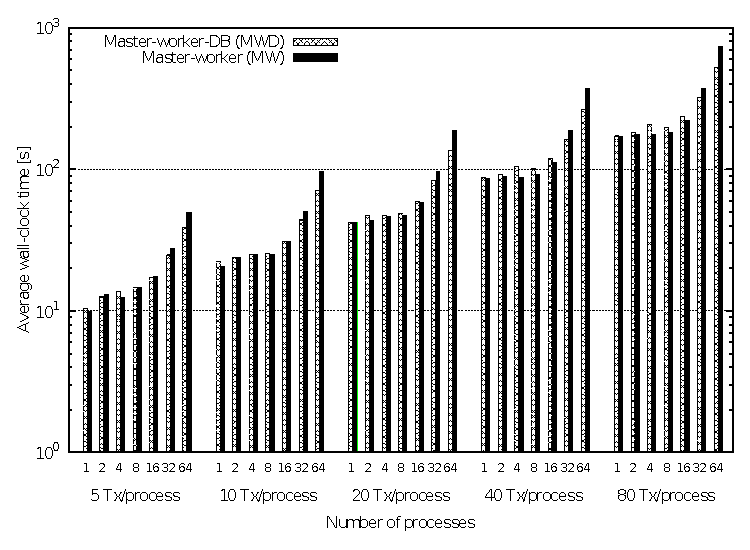
\includegraphics[width=0.8\textwidth]{04-framework_design_and_implementation/img/weak_scaling-time_plot}

\caption{\textit{\emph{Measured wall-clock time for weak-scalability experiments,
featuring MW and MWD setups.}}\textit{ }\textit{\emph{Experiments
allocated one MPI worker process per core.\label{fig:04-Weak_scalability_time}}}}
\end{figure}


\begin{table}
\centering

\caption{\textit{\emph{Running-time gain (in percent) of the simulations for
the weak-scalability of the MWD setup relative to the classic MW approach.\label{tab:04-Weak_scaling-time_gain}}}}


{\small{}}%
\begin{tabular}{cccccccc}
\cmidrule{2-8} 
 & \multicolumn{7}{c}{{\small{Number of cores}}}\tabularnewline\addlinespace
\midrule 
{\small{TX/core}} & {\small{1}} & {\small{2}} & {\small{4}} & {\small{8}} & {\small{16}} & {\small{32}} & {\small{64}}\tabularnewline
\midrule
{\small{5}} & {\small{-11.39}} & {\small{-10.42}} & {\small{-11.14}} & {\small{-0.95}} & {\small{11.75}} & {\small{26.15}} & {\small{32.53}}\tabularnewline
{\small{10}} & {\small{-5.84}} & {\small{-7.78}} & {\small{-7.67}} & {\small{0.91}} & {\small{12.81}} & {\small{33.28}} & {\small{33.55}}\tabularnewline
{\small{20}} & {\small{-8.59}} & {\small{-10.88}} & {\small{-1.04}} & {\small{1.95}} & {\small{14.29}} & {\small{35.23}} & {\small{35.27}}\tabularnewline
{\small{40}} & {\small{-5.26}} & {\small{-6.90}} & {\small{-3.68}} & {\small{-0.67}} & {\small{17.27}} & {\small{36.23}} & {\small{36.65}}\tabularnewline
{\small{80}} & {\small{-5.29}} & {\small{-7.11}} & {\small{-3.20}} & {\small{-0.31}} & {\small{17.94}} & {\small{36.32}} & {\small{36.57}}\tabularnewline
\bottomrule
\end{tabular}
\end{table}


The time measurements observed from the weak-scalability results show
that the classic MW approach performs well for up to four worker processes.
When using eight worker processes, the MW setup is practically equivalent
to the MWD approach, indicating that the master process is being fully
exploited. When increasing the problem size and the number of worker
processes to 16, the running-time gain is already clear, favoring
the MWD configuration. This gain keeps growing, although slower, as
we increase the number of worker processes to 32 and 64, confirming
the hypothesis that in a classic MW approach, the parallel efficiency
is bounded by the capacity of the master process to serve an increasing
number of worker processes. Interestingly, the gain when using 32
and 64 worker processes is almost the same. After further investigation,
the reason for this behavior was found: the new bottleneck was the
LAN being completely saturated by the worker processes. Consequently,
they have to wait for the network resources to become available before
sending or receiving data, which is not the case when running the
MW setup. Therefore, using the MWD approach a hardware constraint
is hit, meaning that the bottleneck is no longer at the implementation
level. Moreover, since the master process is far from overloaded when
serving 64 worker processes, it can be expected that the MWD approach
will keep scaling if a faster network infrastructure is used, e.g.,
10-gigabit Ethernet or InfiniBand.

Certainly, the parallel version of PRATO scales better using the MWD
approach, when challenged with a large number of transmitters (5,120
for the biggest instance) over 64 cores. This fact shows PRATO would
be able to calculate the radio-coverage prediction for real networks
in a feasible amount of time, since many operational radio networks
have already deployed a comparable number of transmitters, e.g., the
3G network within the Greater London Authority area, in the UK~\cite{Number_of_base_stations_in_England}.
For a more in-depth discussion and experimentation about real-world
planning scenarios, see Chapter~\ref{chap:08-Real-world_network_planning}.

Not being able to achieve perfect weak scalability using the MWD setup
is due to a number of factors. Specifically, the overhead time of
the serial sections of the parallel process grows proportionally with
the number of cores, e.g., aggregation of the intermediate results,
although the total contribution of this overhead remains low for large
problem sizes. Moreover, the communication overhead grows linearly
with the number of cores used. Consequently, the findings of Huang
et al. \cite{Huang-Explorations_of_the_implementation_of_a_parallel_IDW_algorithm_in_a_Linux_cluster:2011}
can be confirmed, who concluded that the data-set size should be large
enough for the communication overhead to be hidden by the calculation
time. This ensures profitable parallelization in terms of running-time
reduction.


\subsection{Strong scalability \label{sub:04-Strong_scalability}}

This set of simulations is meant to analyze the impact of increasing
the number of computing cores for a given problem size, i.e., the
number of transmitters deployed over the target area does not change,
but only the number of worker processes used is increased. Here, the
following number of transmitters were tested \{1,280,~2,560,~5,120\},
by gradually doubling the number of workers from 1 to 64 for each
problem size.


\subsubsection*{Results}

\begin{figure}
\centering

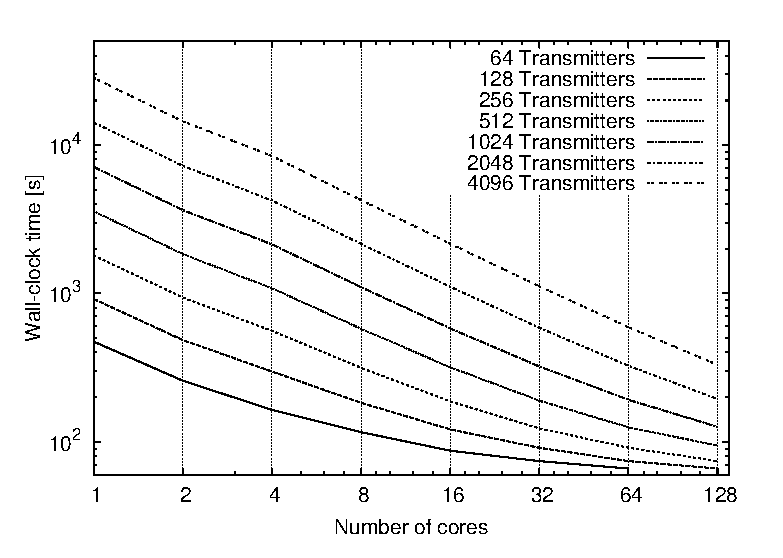
\includegraphics[width=0.8\columnwidth]{04-framework_design_and_implementation/img/strong_scaling-time_plot}

\caption{\textit{\emph{Measured wall-clock time for strong-scalability experiments,
featuring MW and MWD setups.}}\textit{ }\textit{\emph{Experiments
assigned one MPI worker process per core. \label{fig:04-Strong_scalability_time}}}}
\end{figure}


Similar to the weak-scalability experiments, the time measurements
plotted in Figure~\ref{fig:04-Strong_scalability_time} show that,
when applying a classic MW approach, the \textit{\emph{running-time
reduction}} starts flattening if more than eight worker processes
were used. Moreover, the running times for 16, 32 and 64 worker processes
are the same, i.e., they do not improve due to the master process
being \textit{\emph{saturated}}. In contrast, when using the proposed
MWD technique, the running-time reduction improves for up to 32 worker
processes, after which there is no further improvement since the network
was being fully exploited. These results clearly show that when applying
parallelization using a larger number of worker processes, the master
process becomes the bottleneck of the MW approach. When using the
MWD configuration, a steady running-time reduction is observed, until
a hardware constraint is hit, e.g., the network infrastructure.

The overhead of sending/receiving asynchronous messages in order to
support heterogeneous systems was also measured. It was found that
this overhead never exceeds 0.02\% of the total running time for the
MW experiments, and 0.01\% for the MWD experimental set.


\subsubsection{Speedup}

In order to further analyze how well the PRATO scales using the MW
and MWD approaches, the performance of the parallel implementation
in terms of its speedup was measured, which is defined as:

\begin{equation}
S(NP)=\frac{execution\, time\, for\, base\, case}{execution\, time\, for\, NP\, cores},\label{eq:04-Speedup}
\end{equation}


\noindent where $NP$ is the number of cores executing the worker
processes. The parallel implementation running on only one core was
the base case for comparisons. The serial implementation is not a
good base comparison for the parallel results as it does not reuse
the resources between each transmitter-coverage calculation and it
does not overlap the I/O operations with the transmitter computations.
In practice, this means that several concatenated runs of the serial
version would be considerably slower than the single-worker configuration.

\begin{figure}
\begin{minipage}[t]{0.48\textwidth}%
\centering

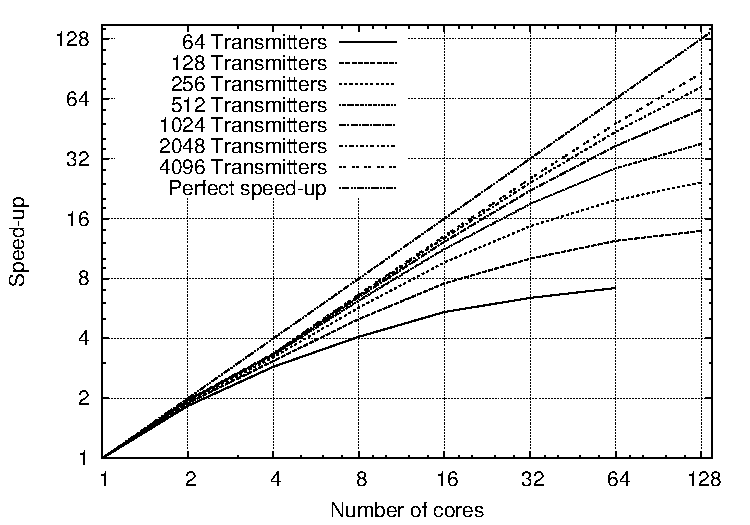
\includegraphics[width=1\columnwidth]{04-framework_design_and_implementation/img/strong_scaling-speedup_plot}

\caption{\textit{\emph{Average speedup for the strong-scalability experiments.
\label{fig:04-Strong_scalability_speedup}}}}
%
\end{minipage}\hfill{}%
\begin{minipage}[t]{0.48\textwidth}%
\centering

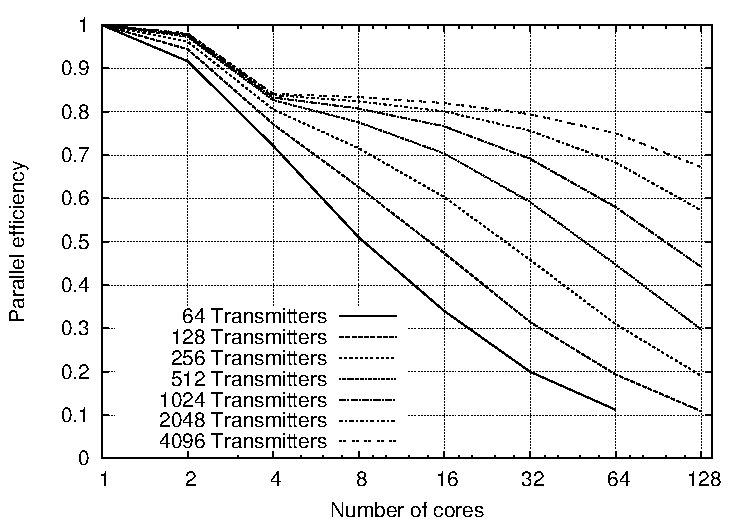
\includegraphics[width=1\columnwidth]{04-framework_design_and_implementation/img/strong_scaling-efficiency_plot}

\caption{\textit{\emph{Average parallel efficiency for the strong-scalability
experiments.}}\textit{ }\textit{\emph{\label{fig:04-Strong_scalability_efficiency}}}}
%
\end{minipage}
\end{figure}


Using the speedup metric, linear scaling is achieved when the obtained
speedup is equal to the total number of processors used. However,
it should be noted that a perfect speedup is almost never achieved,
due to the existence of serial stages within an algorithm and the
communication overhead of the parallel implementation.

Figure~\ref{fig:04-Strong_scalability_speedup} shows the average
speedup of the parallel implementation for up to 64 worker processes,
using the standard MW method and the proposed MWD approach. The average
speedup was calculated for the three different problem instances,
i.e., 1,280, 2,560, and 5,120 transmitters deployed over the target
area. The number of transmitters used in these problem sizes is comparable
to several real-world radio networks that were already deployed in
England, e.g., Hampshire County with 227 BSs, West Midlands with 414
BSs, and Greater London Authority with 1,086 BSs \cite{Number_of_base_stations_in_England}.
Note that it is common for a single base station to host multiple
transmitters. 

The plotted average speedup clearly shows the minimal overhead of
the MWD approach when using a small number of worker processes. This
overhead accounts for the final aggregation of the intermediate results
at the DB, which in the MW configuration is performed along worker
processing. Like before, the DB component allows the parallel implementation
to fully exploit the available computing resources when deploying
a larger number of worker processes, until the network-capacity limit
is met. Of course, these results are directly correlated with the
wall-clock times shown in Figure~\ref{fig:04-Strong_scalability_time}.


\subsubsection{Efficiency}

Another measure to study how well PRATO utilizes the available computing
resources considers the parallel efficiency of the implementation.
The definition of parallel efficiency is as follows:

\begin{equation}
E(NP)=\frac{S(NP)}{NP},
\end{equation}


\noindent where $S(NP)$ is the speedup as defined in Equation~(\ref{eq:04-Speedup}),
and $NP$ is the number of cores executing worker processes. Figure~\ref{fig:04-Strong_scalability_efficiency}
shows the average parallel efficiency of the parallel implementation
for different problem sizes, as the number of processing cores was
increased. Like for the speedup measure, the average parallel efficiency
from the same problem instances was calculated.

The ideal case for a parallel application would be to utilize all
the available computing resources, in which case the parallel efficiency
would always be equal to one as the core count increases. From the
plot in Figure~\ref{fig:04-Strong_scalability_efficiency}, it can
be observed that the efficiency of the MWD approach is better than
in the MW case for larger number of processes, and as long as there
was available capacity at the LAN level. In accordance to the previous
analysis, the under utilization of the computing resources is more
significant when the master process is overloaded (in the MW case)
than when the network infrastructure is saturated (in the MWD case).
The lower efficiency is directly proportional to the number of idle
worker processes that wait either for the master process (MW case)
or for network access (MWD case).

Overall, the experimental results confirm that the objective of fully
exploiting the available hardware resources is accomplished when applying
the presented MWD approach, thus improving the scalability and efficiency
of PRATO when compared to a traditional MW technique.




\section{Summary \label{sec:04-Summary}}

PRATO, a parallel radio-coverage prediction tool for radio networks,
has been presented in this chapter. The tool is intended to be used
for radio-network planning analysis and decision support. Its high-performance
capabilities make it ideal for automatic-optimization tasks that require
a large number of evaluations.

The parallel implementaion of PRATO includes a novel parallel technique
for master-worker configurations. The introduced MWD technique, which
combines the use of a DB system with a work-pool approach, delivers
improved performance when compared with a traditional MW setup. Moreover,
the presented system provides parallel and asynchronous computation
that is completely independent of the GIS used, in this case the GRASS
environment. Consequently, a GIS installation is only needed on the
master node, thus simplifying the required system setup and greatly
enhancing the applicability of this methodology in different environments.

The extensive simulations, performed on the DEGIMA cluster of the
Nagasaki Advanced Computing Center, were analyzed to determine the
level of scalability of the implementation, as well as the impact
of the presented methods for parallel-algorithm design aimed at spatial-data
processing. The conducted analyses show that when using the MWD approach,
PRATO is able to calculate the radio-coverage prediction of real-world
radio networks in a reduced amount of time. Moreover, the experimental
results show that PRATO has a better scalability when using the MWD
approach than the standard MW setup, since it is able to completely
saturate the network infrastructure of the computer cluster. These
promising results also show the great potential of the MWD approach
for parallelizing different time-consuming tasks dealing with spatial
data, where DBs form an intrinsic part of almost all GIS. Furthermore,
the automatic optimization of radio networks, where a large number
of radio-propagation predictions take part in the evaluation step
of the optimization process, can also an benefit from the improved
performance of PRATO. Indeed, this last point will be further discussed
and validated in the following chapters.

The performance of the worker processes has been additionally improved
by including the implementation of the radio-propagation algorithm
on GPU. The use of GPU hardware is optional, i.e., it is exploited
only if it is available on the computing nodes that host the worker
processes.

To the best of the author's knowledge, neither the MWD parallel technique
nor the parallel implementation of the radio-prediction algorithm
as presented in this chapter, have yet been described in the related
literature.
